\documentclass[12pt,a4paper]{article}
\usepackage[utf8]{inputenc}
\usepackage{graphicx}
\usepackage{float}
\usepackage{booktabs}
\usepackage{longtable}
\usepackage{geometry}
\usepackage{amsmath}
\usepackage{hyperref}
\usepackage{multirow}
\usepackage{array}
\usepackage{caption}
\usepackage{subcaption}

\geometry{margin=1in}
\graphicspath{{figures/}}

% Optimize image loading - simpler settings
\DeclareGraphicsExtensions{.png,.pdf,.jpg}

\title{Crash Pattern Analysis: Temporal and Geographic Variations\\
in Urban and Rural Areas of Victoria}
\author{Your Name\\
Big Data Project}
\date{\today}

\begin{document}

\maketitle

\begin{abstract}
This study investigates how crash frequency, severity, and type vary by time of day, day of week, and season, and how these patterns differ between urban and rural areas in Victoria. Using a comprehensive dataset of 187,018 crashes, we employ exploratory data analysis, statistical testing, and machine learning methods to identify high-risk periods and environmental factors. Results reveal significant differences between urban and rural crash patterns, with rural areas experiencing fatal crash rates approximately four times higher than urban areas. Night/late night periods and Friday emerge as the highest risk temporal periods, particularly in rural areas. Machine learning models achieve 98.3\% accuracy in predicting fatal crashes, with accident type, speed zone, and area type identified as the most important risk factors.
\end{abstract}

\tableofcontents
\newpage

\section{Introduction}

\subsection{Background}
Road traffic crashes represent a significant public health concern, causing substantial mortality and morbidity worldwide. Understanding the temporal and geographic patterns of crashes is crucial for developing effective prevention strategies and resource allocation. Previous research has identified differences in crash characteristics between urban and rural settings, but comprehensive analysis of temporal patterns across these contexts remains limited.

\subsection{Research Objectives}
This project aims to:
\begin{enumerate}
    \item Investigate how crash frequency, severity, and type vary by time of day, day of week, and season
    \item Compare crash patterns between urban and rural areas in Victoria
    \item Identify high-risk periods and environmental factors associated with severe crashes
    \item Develop predictive models for crash severity using statistical and machine learning methods
\end{enumerate}

\subsection{Research Question}
How do crash frequency, severity, and type vary by time of day, day of week, and season, and how do these patterns differ between urban and rural areas in Victoria?

\section{Data Description}

\subsection{Dataset Overview}
The analysis utilizes crash data from Victoria, Australia, comprising 187,018 recorded accidents. The dataset includes information from multiple related tables:

\begin{itemize}
    \item \textbf{accident}: Primary crash data with 188,006 records containing temporal, severity, and crash type information
    \item \textbf{node}: Geographic classification data providing urban/rural categorization
    \item \textbf{person}: Person-level severity information for 438,984 individuals
    \item \textbf{atmospheric\_cond}: Environmental condition data for 190,417 records
    \item \textbf{road\_surface\_cond}: Road surface condition data
\end{itemize}

\subsection{Data Preprocessing}
The raw data underwent comprehensive cleaning and preparation:
\begin{itemize}
    \item Date and time parsing from character strings
    \item Factor conversion for categorical variables
    \item Missing data handling and imputation where appropriate
    \item Creation of derived variables (hour groups, season, area type classification)
    \item Data joining across multiple tables using accident identifiers
\end{itemize}

\subsection{Key Variables}
\begin{itemize}
    \item \textbf{Temporal}: Time of day (hour, hour groups), day of week, season
    \item \textbf{Geographic}: Area type (Urban/Rural classification)
    \item \textbf{Severity}: Numeric severity codes (1=Fatal, 2=Serious, 3=Minor, 4=Property damage)
    \item \textbf{Crash Type}: Categorical accident type descriptions
    \item \textbf{Environmental}: Atmospheric conditions, road surface conditions
    \item \textbf{Traffic}: Speed zone, number of vehicles
\end{itemize}

\section{Methodology}

\subsection{Exploratory Data Analysis}
Initial exploratory analysis focused on understanding the distribution of crashes across temporal and geographic dimensions. Visualizations were created to examine:
\begin{itemize}
    \item Crash frequency patterns by time, day, and season
    \item Severity distributions and patterns
    \item Crash type distributions
    \item Environmental factor associations
\end{itemize}

\subsection{Statistical Analysis}
Statistical testing employed:
\begin{itemize}
    \item Chi-square tests for categorical associations (frequency, severity, crash type patterns)
    \item Fisher's exact test for fatal crash rate comparisons (suitable for small cell counts)
    \item Cramér's V for effect size measurements
    \item Significance level: $\alpha = 0.05$
\end{itemize}

\subsection{Machine Learning Analysis}
Machine learning approaches included:
\begin{itemize}
    \item \textbf{Binary Classification}: Logistic regression and random forest for fatal crash prediction
    \item \textbf{Multi-class Classification}: Random forest for severity category prediction
    \item \textbf{Separate Models}: Urban and rural-specific models to capture area-specific patterns
    \item Model evaluation using train/test split (70/30) and accuracy metrics
    \item Feature importance analysis using random forest mean decrease Gini
\end{itemize}

\section{Exploratory Data Analysis}

\subsection{Crash Frequency Patterns}

Figure \ref{fig:freq_hour} shows crash frequency by hour of day, revealing distinct patterns between urban and rural areas. Urban crashes show clear morning and afternoon rush hour peaks, while rural crashes demonstrate more consistent distribution throughout the day.

\begin{figure}[htbp]
    \centering
    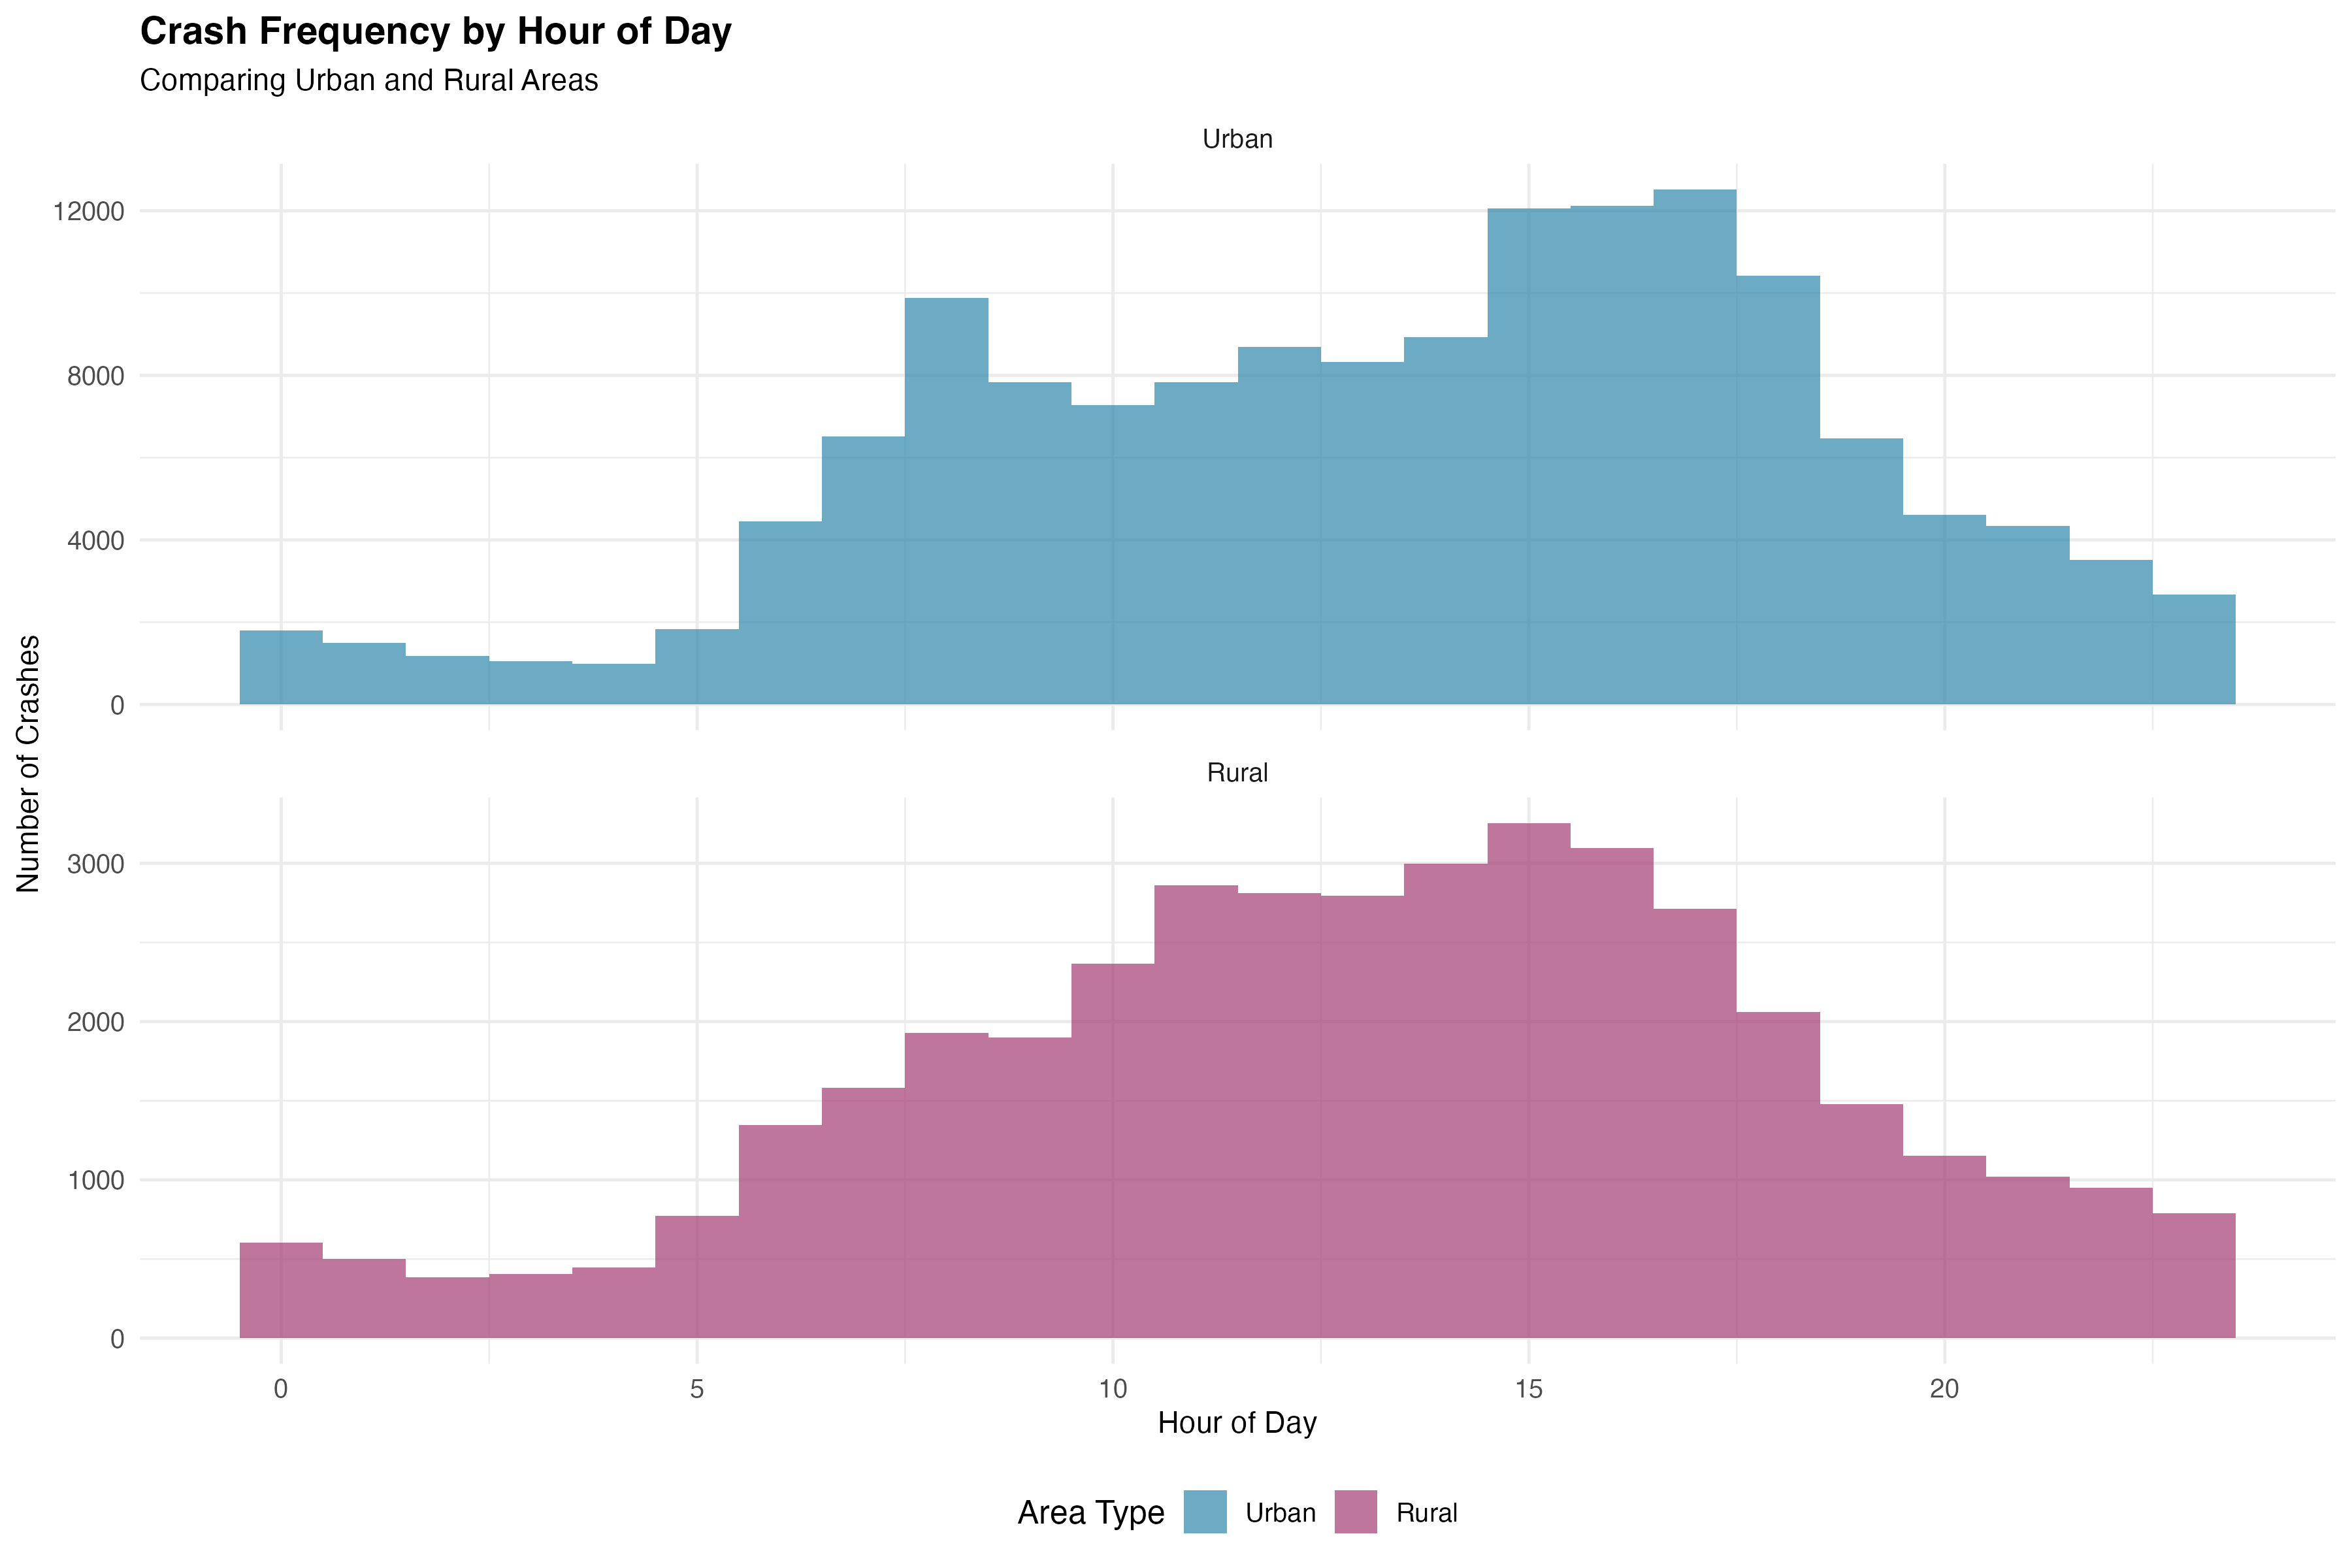
\includegraphics[width=0.7\textwidth]{01_frequency_by_hour_urban_rural.png}
    \caption{Crash frequency by hour of day, comparing urban and rural areas}
    \label{fig:freq_hour}
\end{figure}

The time period analysis indicates that afternoon rush hours (15-18) represent the peak period for both urban and rural crashes, though urban areas show higher absolute numbers. % Figure \ref{fig:freq_time} commented for faster compilation

% \begin{figure}[htbp]
%     \centering
%     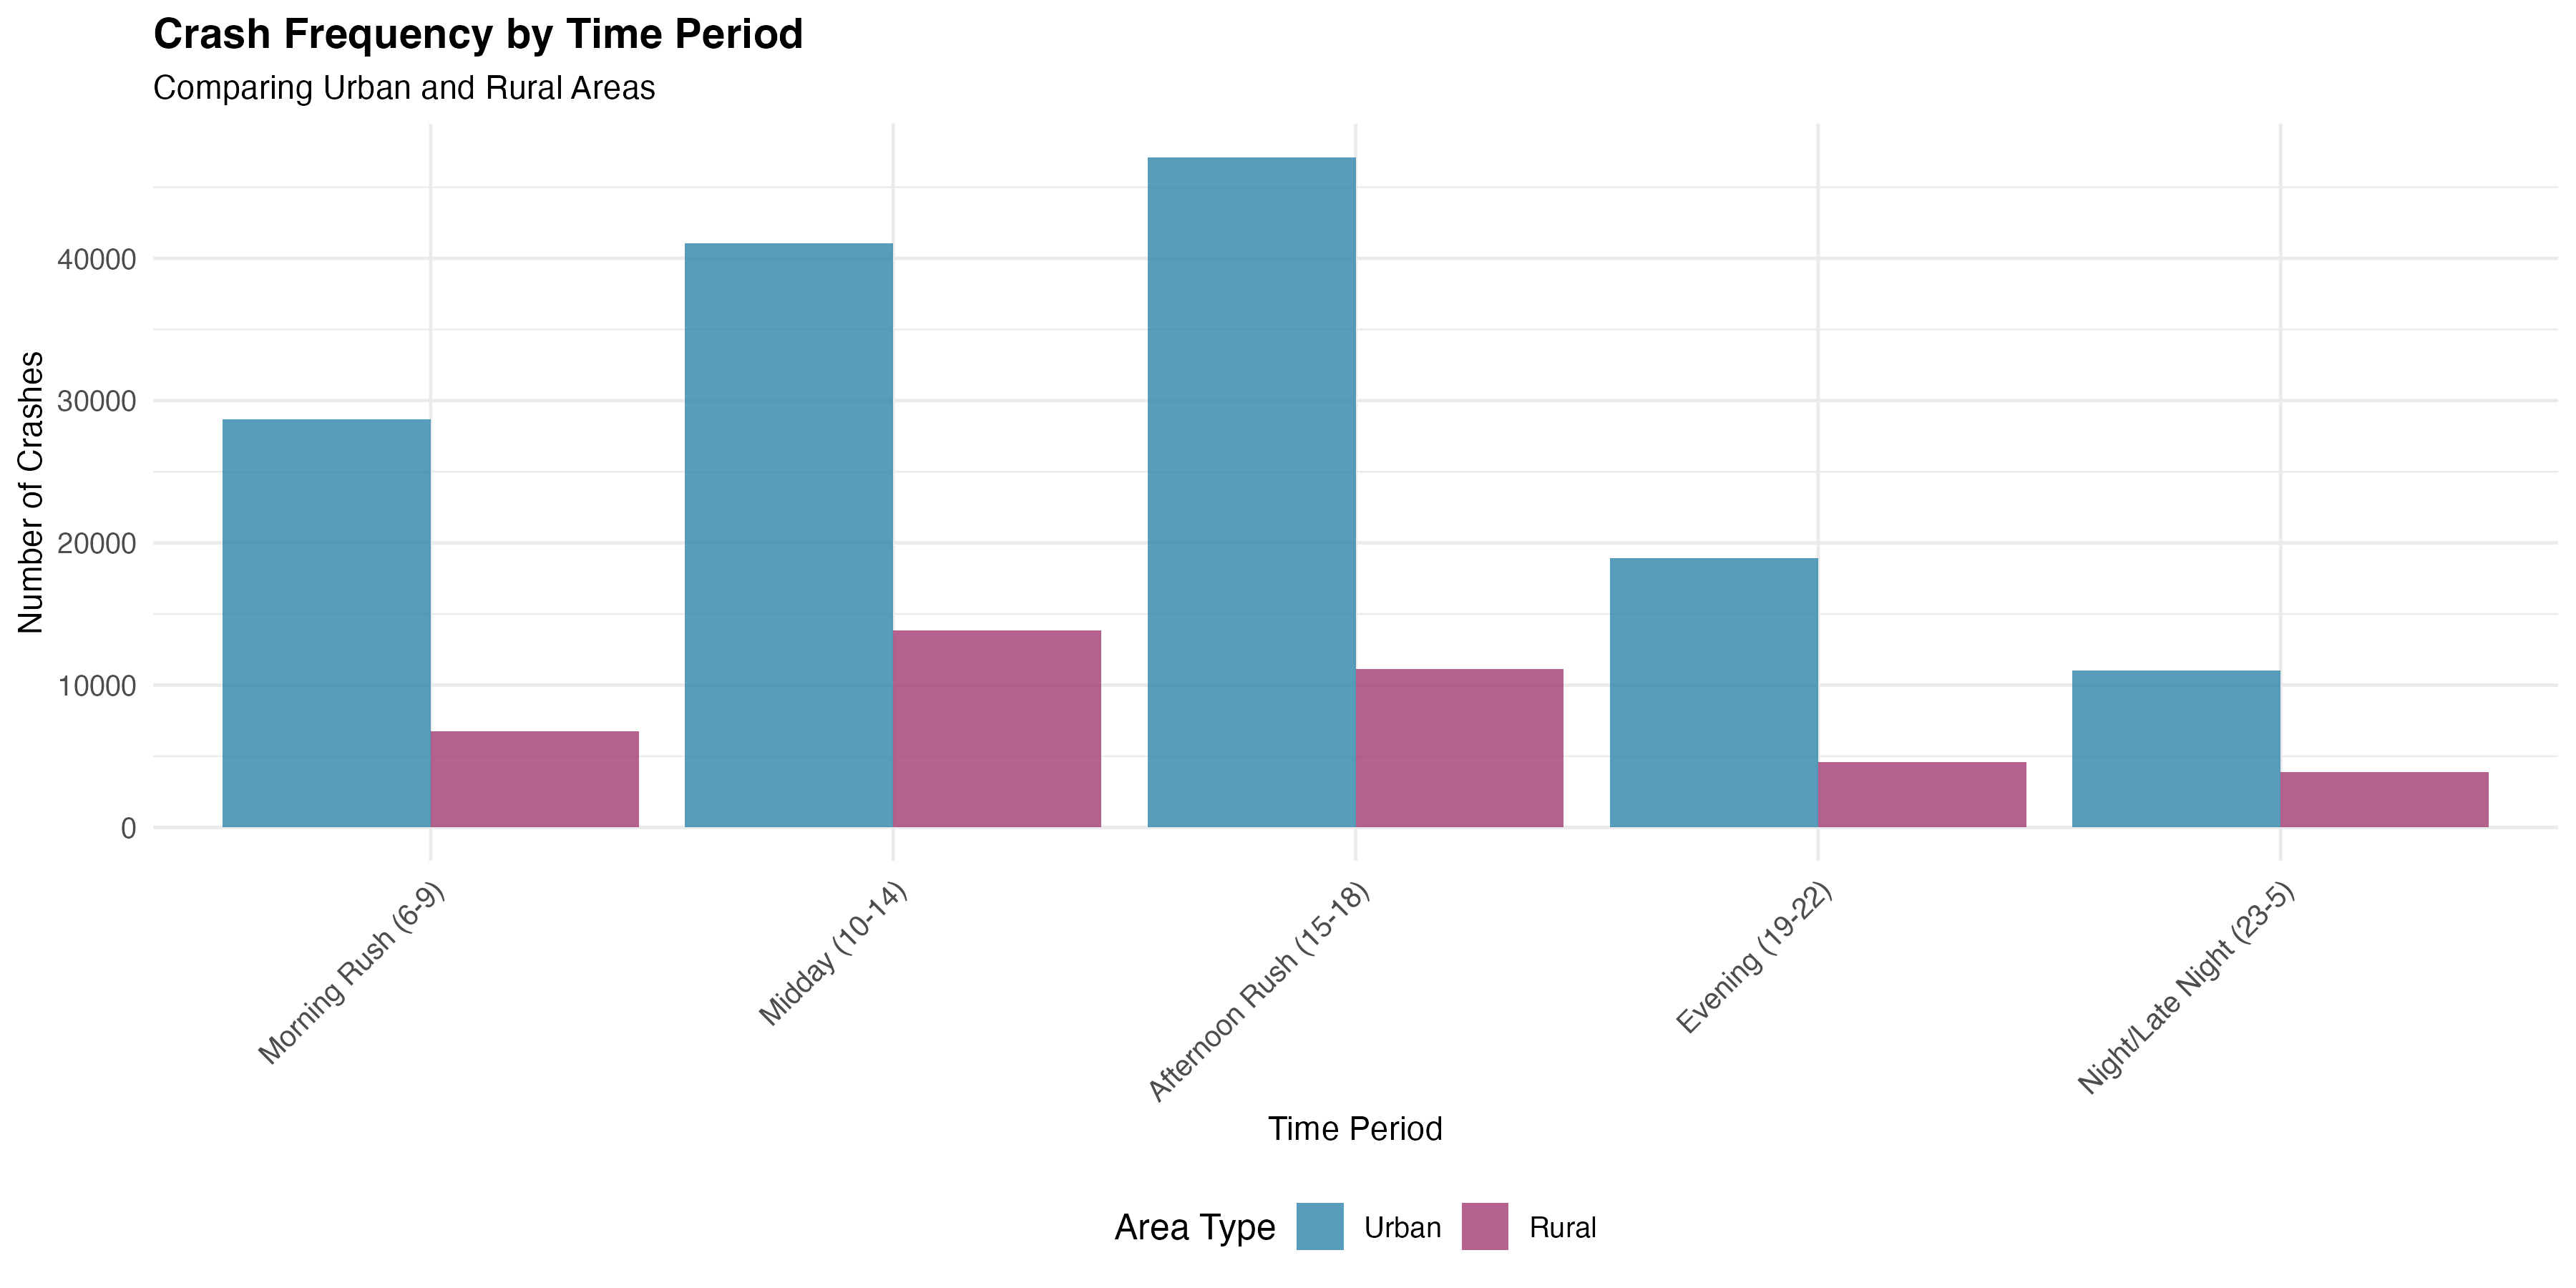
\includegraphics[width=0.7\textwidth]{01_frequency_by_time_group_urban_rural.png}
%     \caption{Crash frequency by time period groups}
%     \label{fig:freq_time}
% \end{figure}

Day of week patterns reveal Friday as the day with highest crash frequency in both urban and rural areas, with urban areas consistently showing higher volumes throughout the week. % Figure \ref{fig:freq_day} commented for faster compilation

% \begin{figure}[htbp]
%     \centering
%     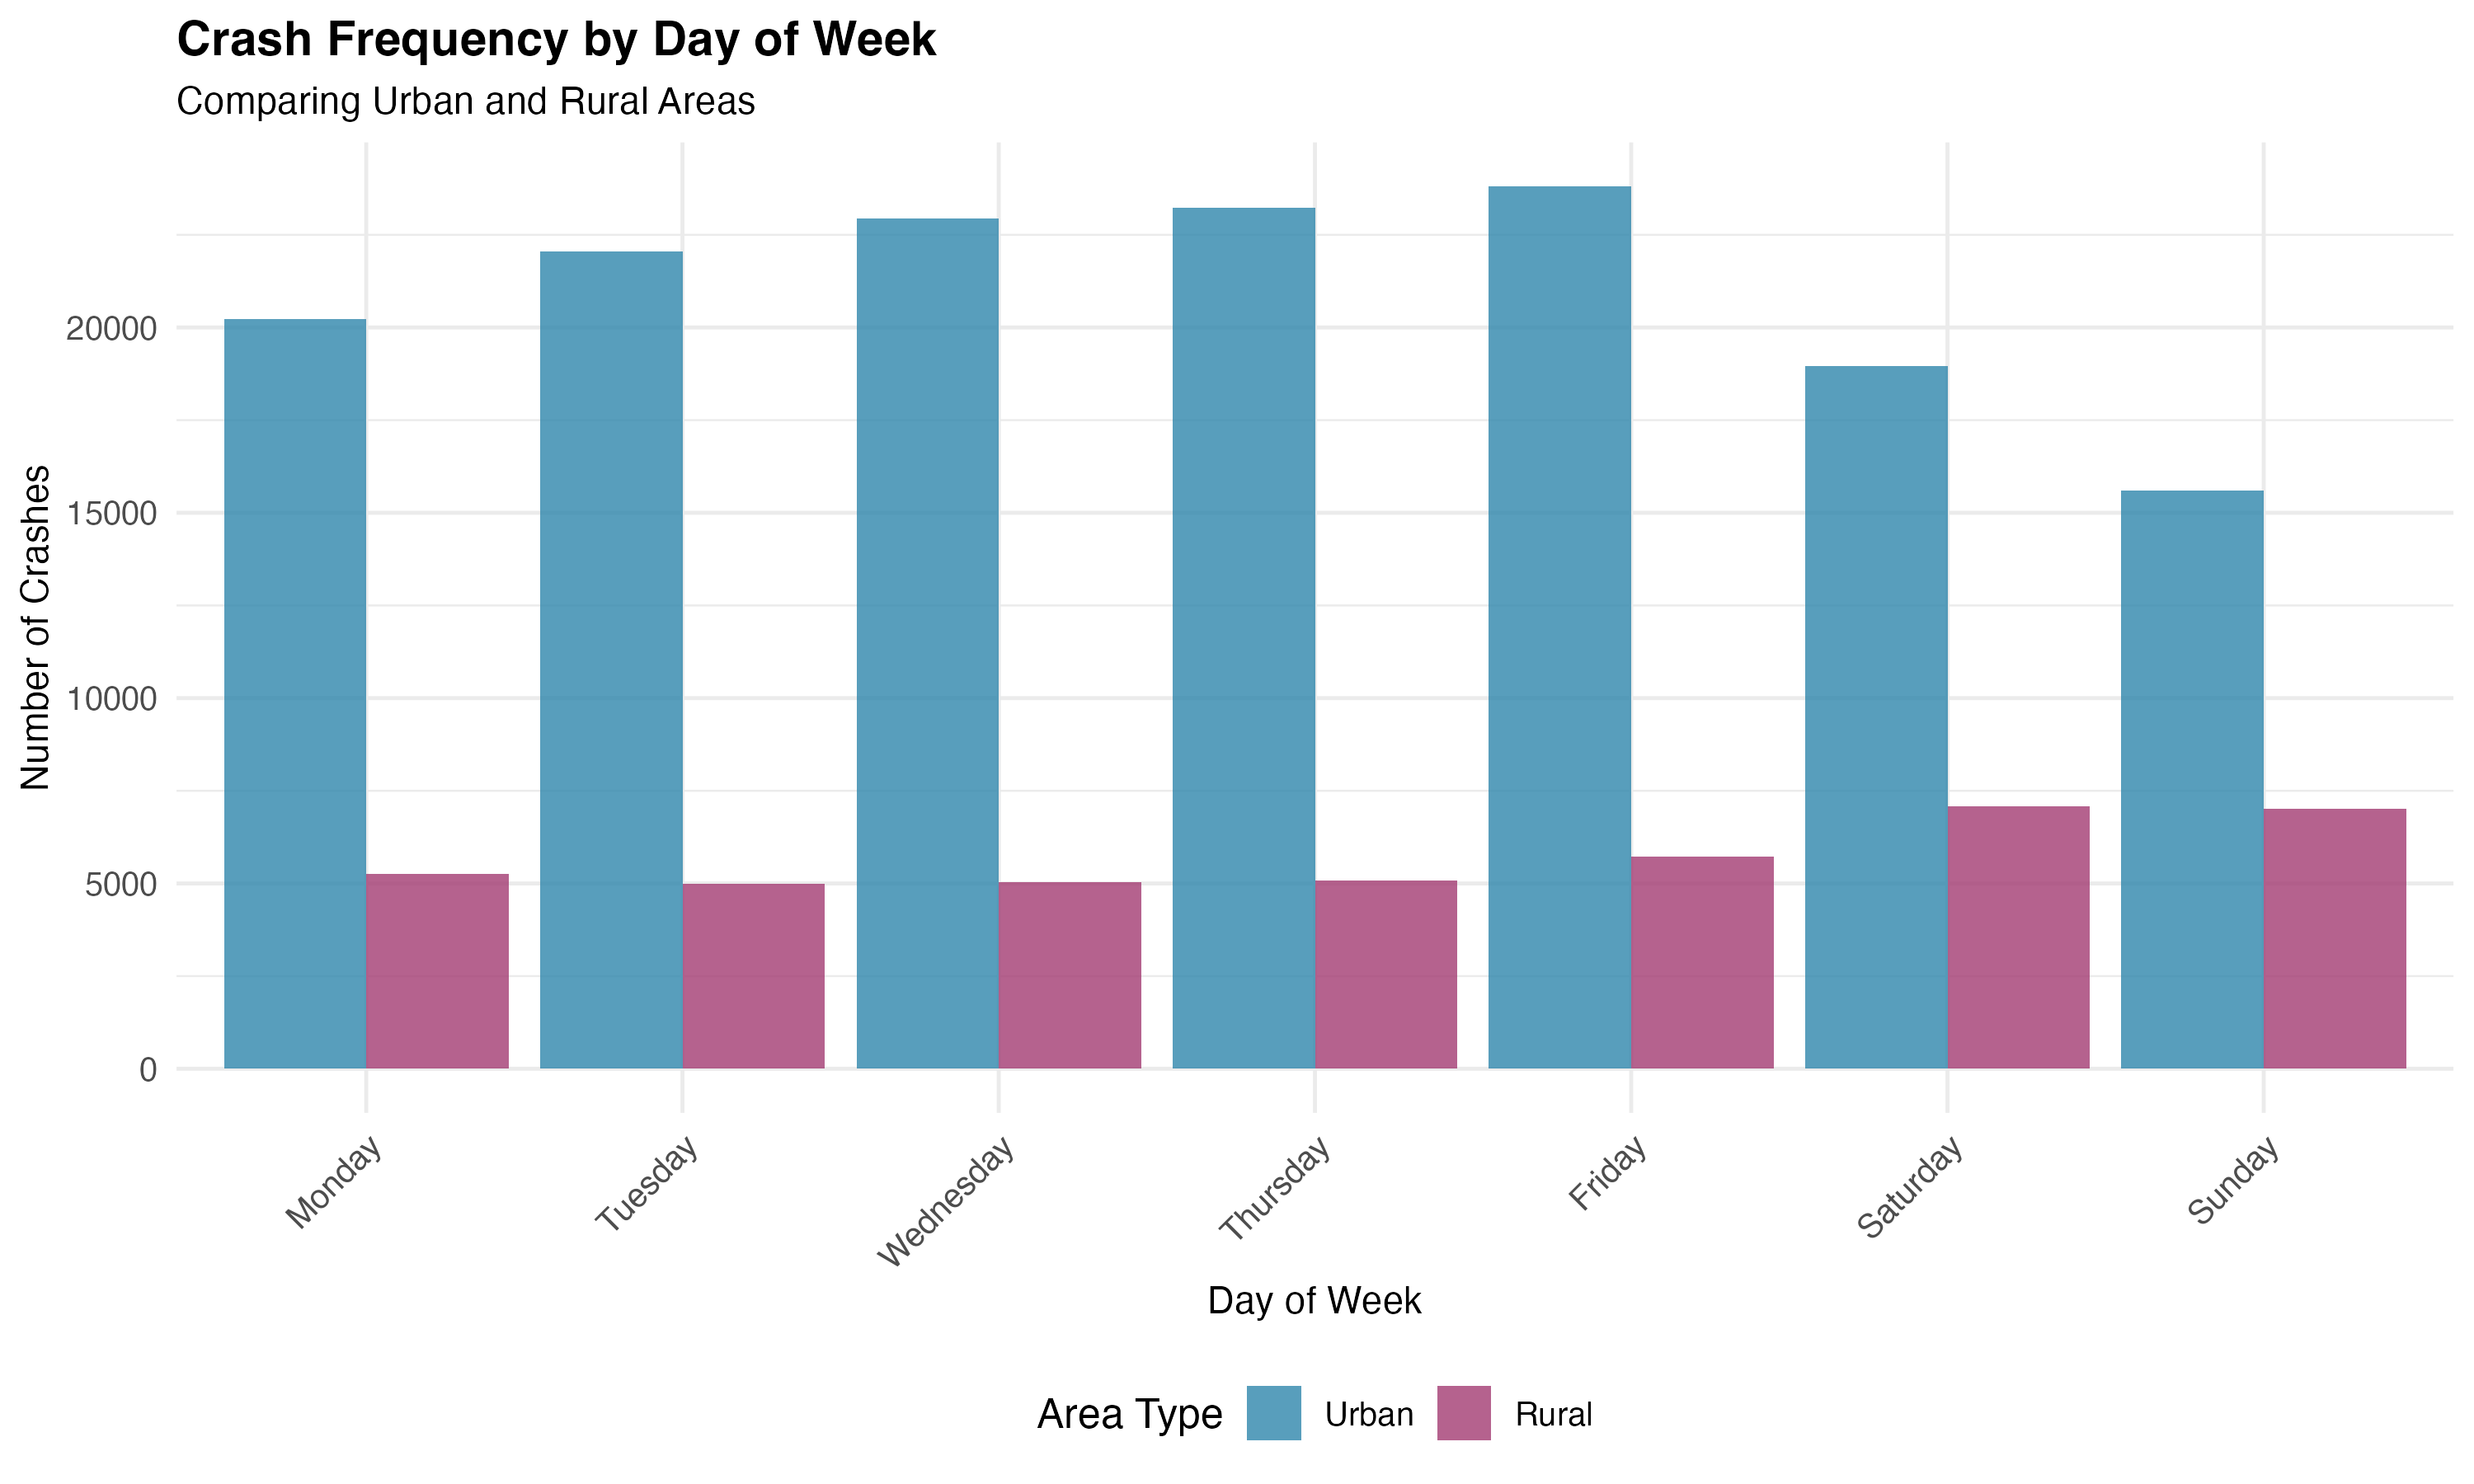
\includegraphics[width=0.7\textwidth]{01_frequency_by_day_week_urban_rural.png}
%     \caption{Crash frequency by day of week}
%     \label{fig:freq_day}
% \end{figure}

Seasonal analysis shows relatively consistent crash frequencies across seasons, with minor variations between urban and rural areas. % Figure \ref{fig:freq_season} commented for faster compilation

% \begin{figure}[htbp]
%     \centering
%     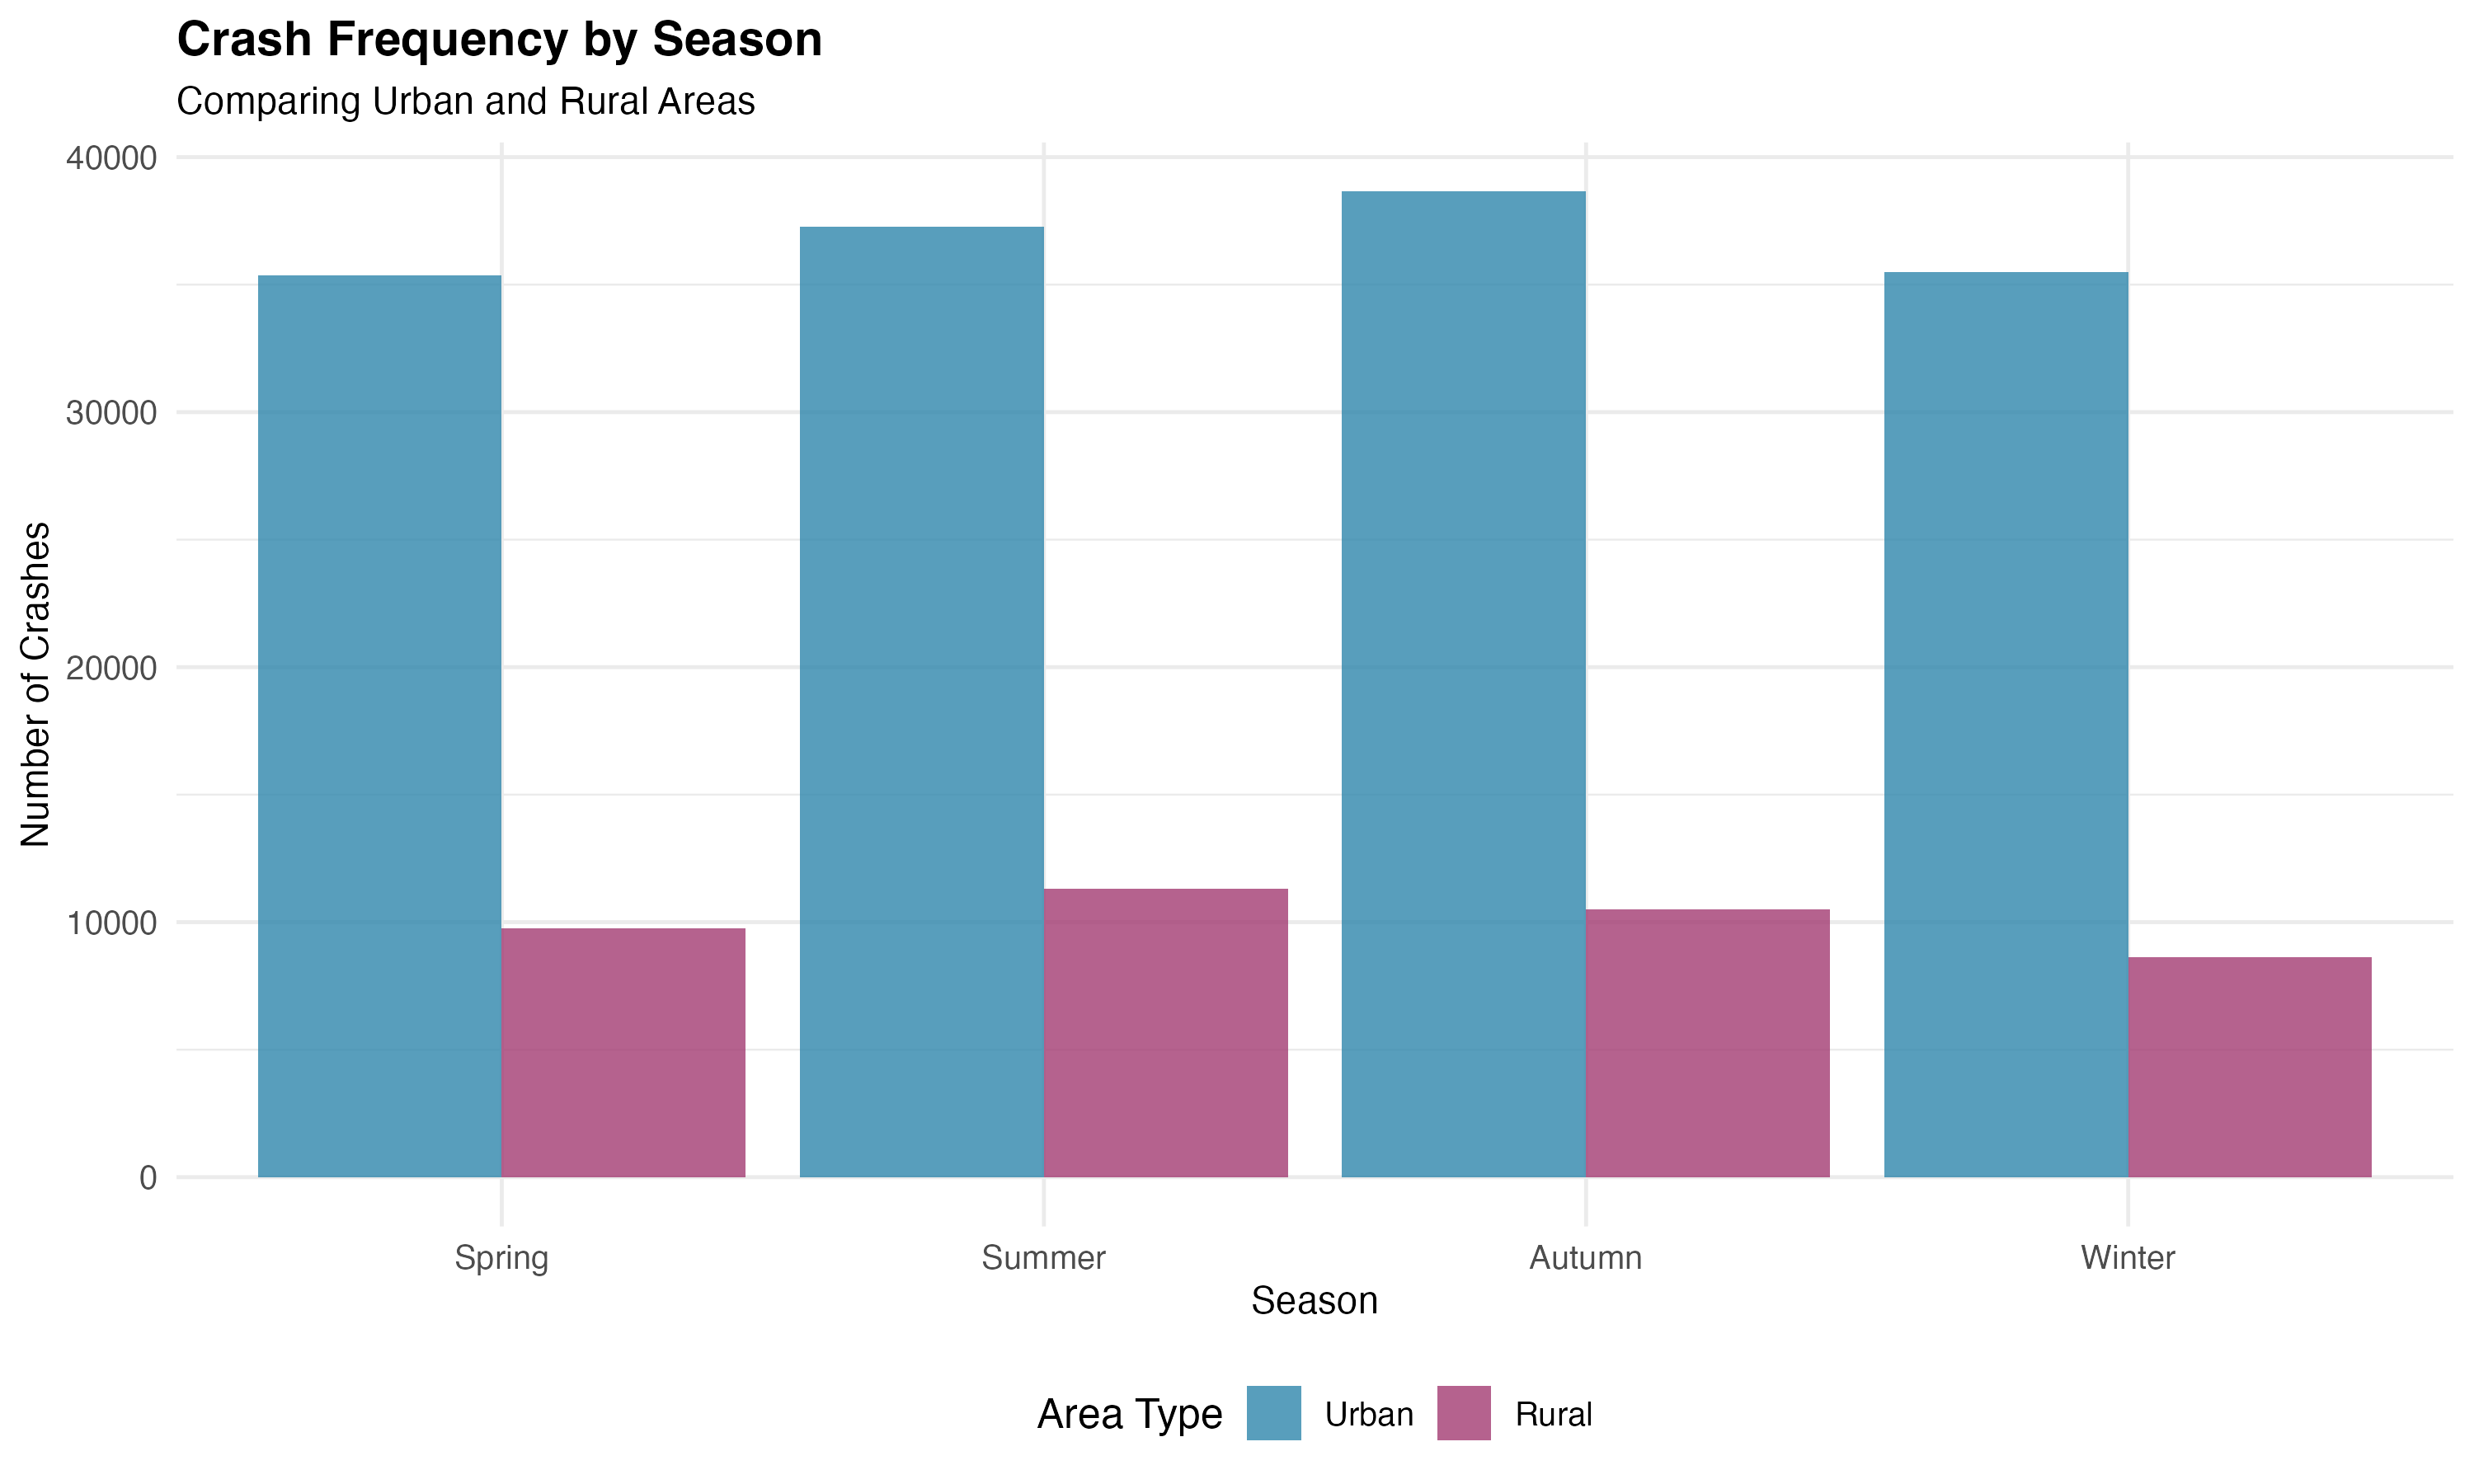
\includegraphics[width=0.7\textwidth]{01_frequency_by_season_urban_rural.png}
%     \caption{Crash frequency by season}
%     \label{fig:freq_season}
% \end{figure}

\subsection{Severity Analysis}

The overall severity distribution (Figure \ref{fig:severity_dist}) reveals substantial differences between urban and rural areas. Rural areas show a significantly higher proportion of fatal and serious crashes compared to urban areas.

\begin{figure}[htbp]
    \centering
    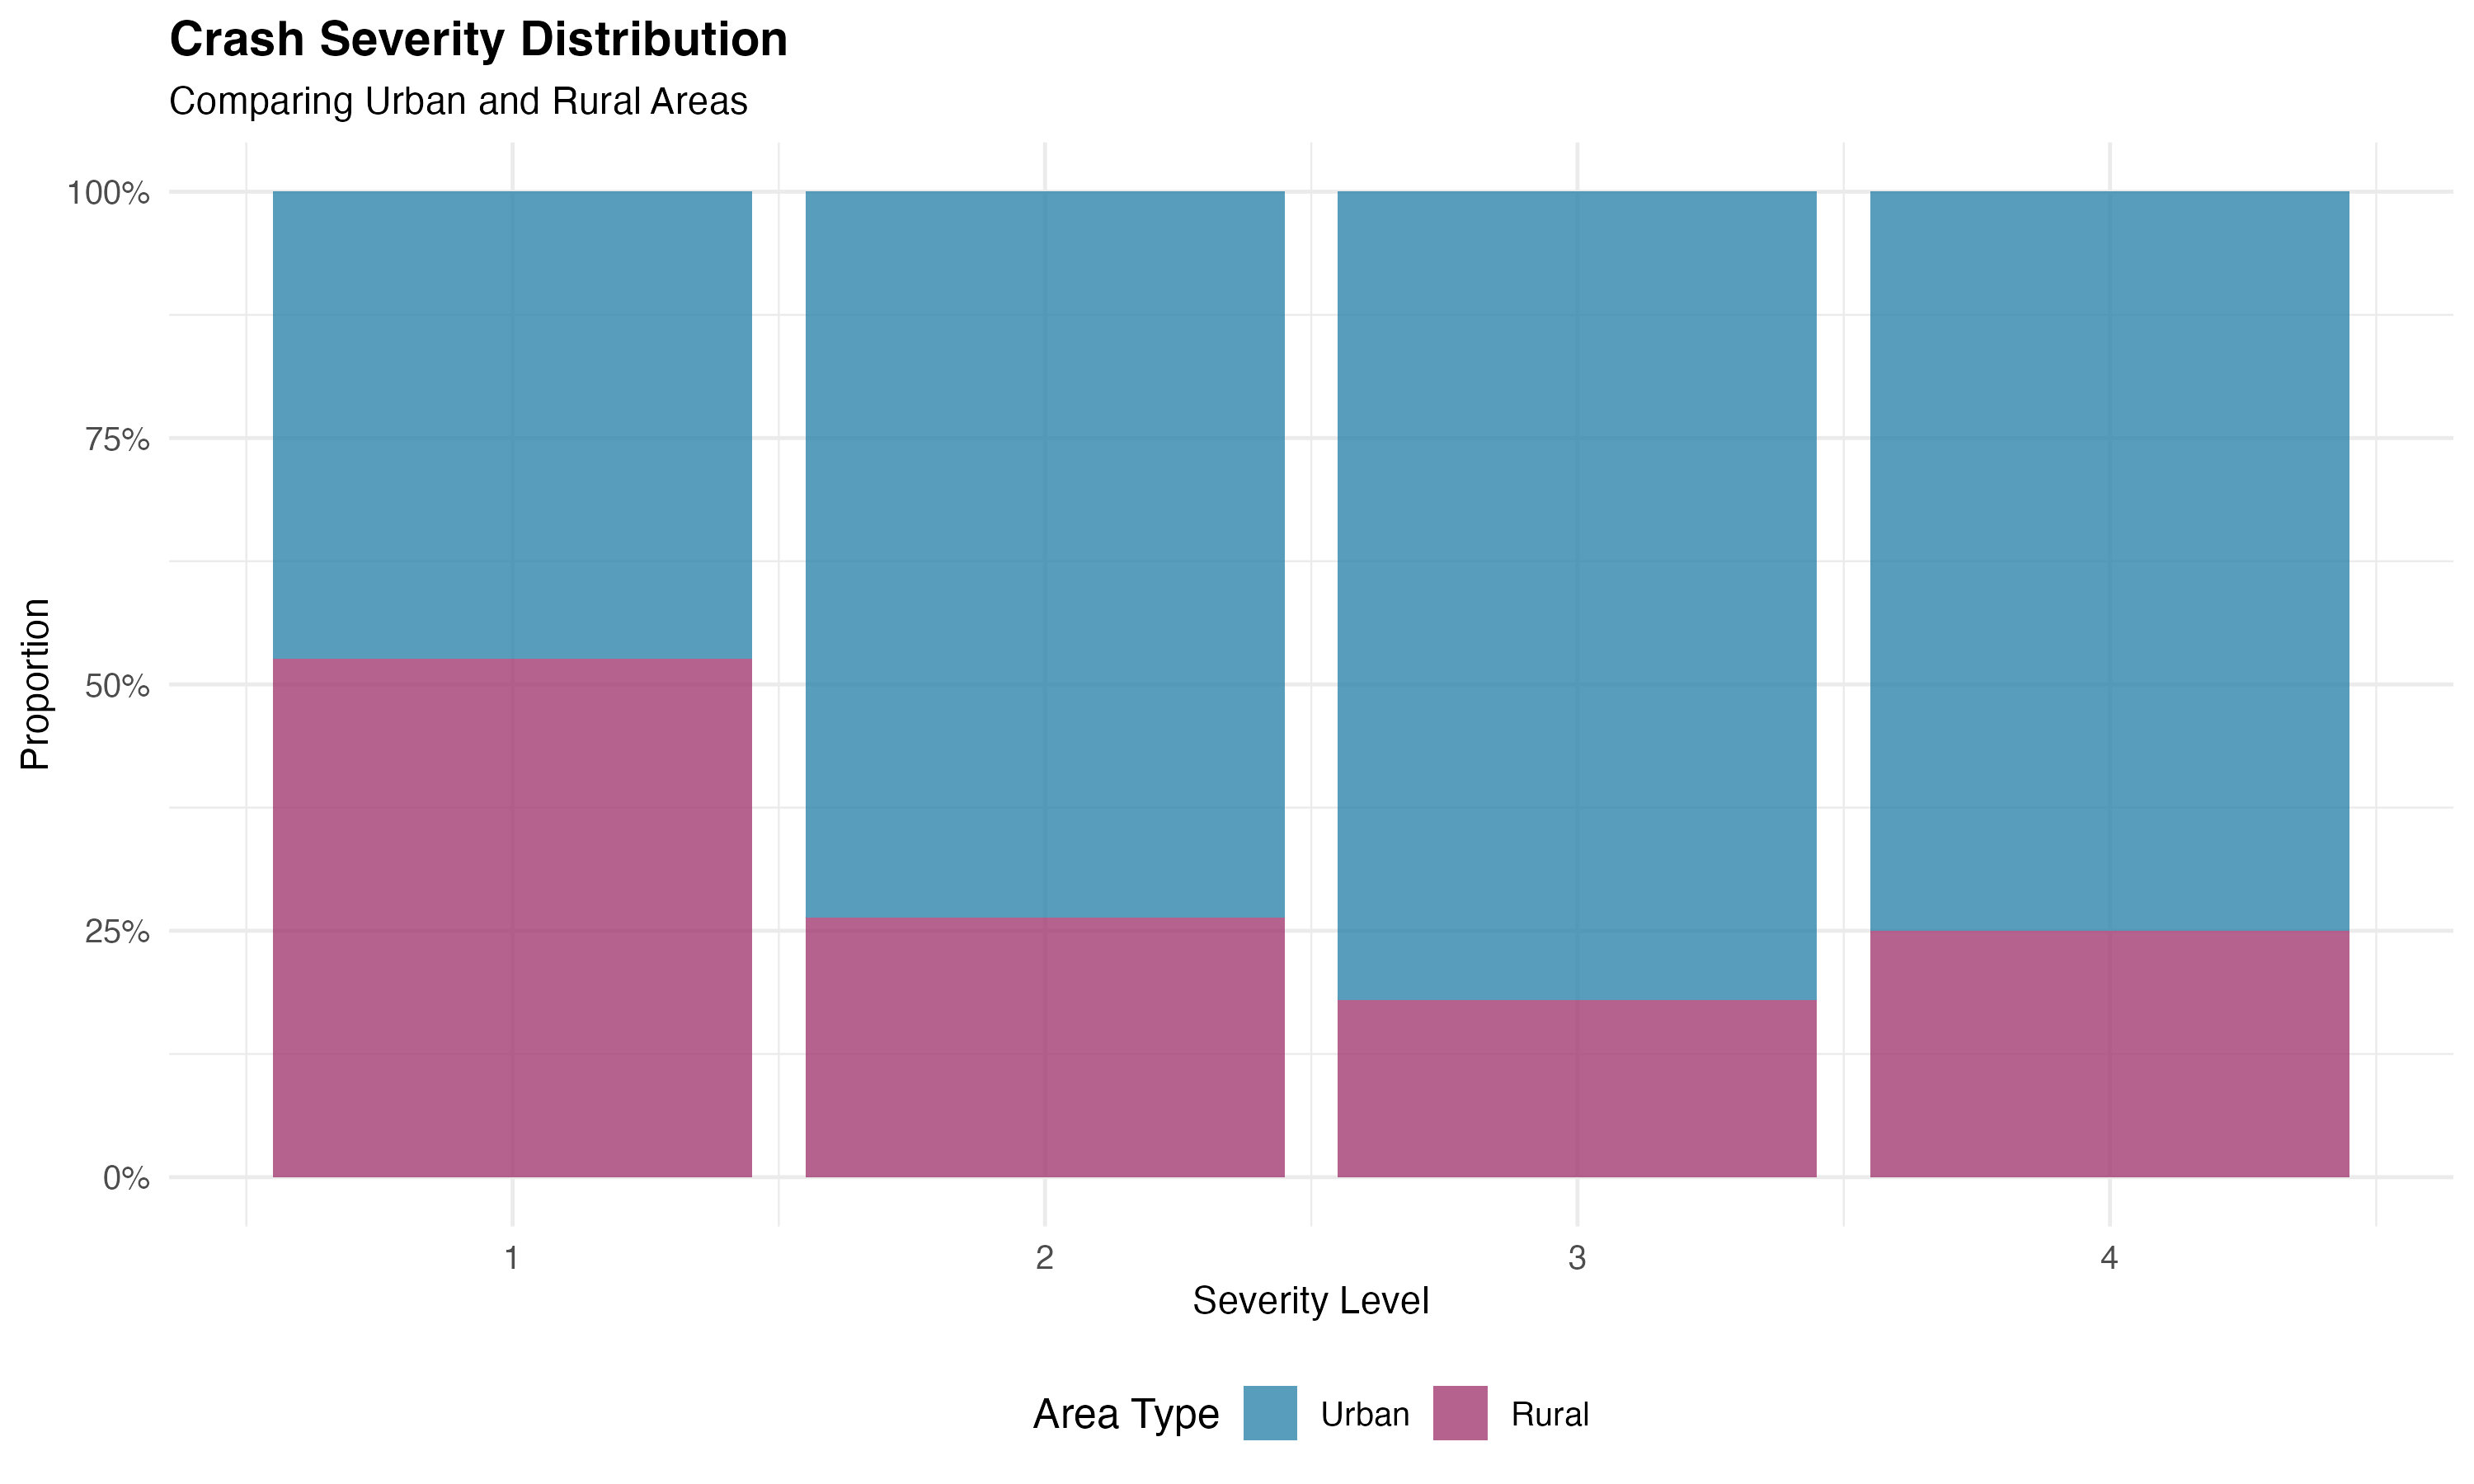
\includegraphics[width=0.7\textwidth]{02_severity_distribution_urban_rural.png}
    \caption{Overall severity distribution comparing urban and rural areas}
    \label{fig:severity_dist}
\end{figure}

Severity patterns by time period indicate that night/late night hours show the highest proportion of severe crashes, particularly in rural areas. % Figure \ref{fig:severity_time} commented for faster compilation

% \begin{figure}[htbp]
%     \centering
%     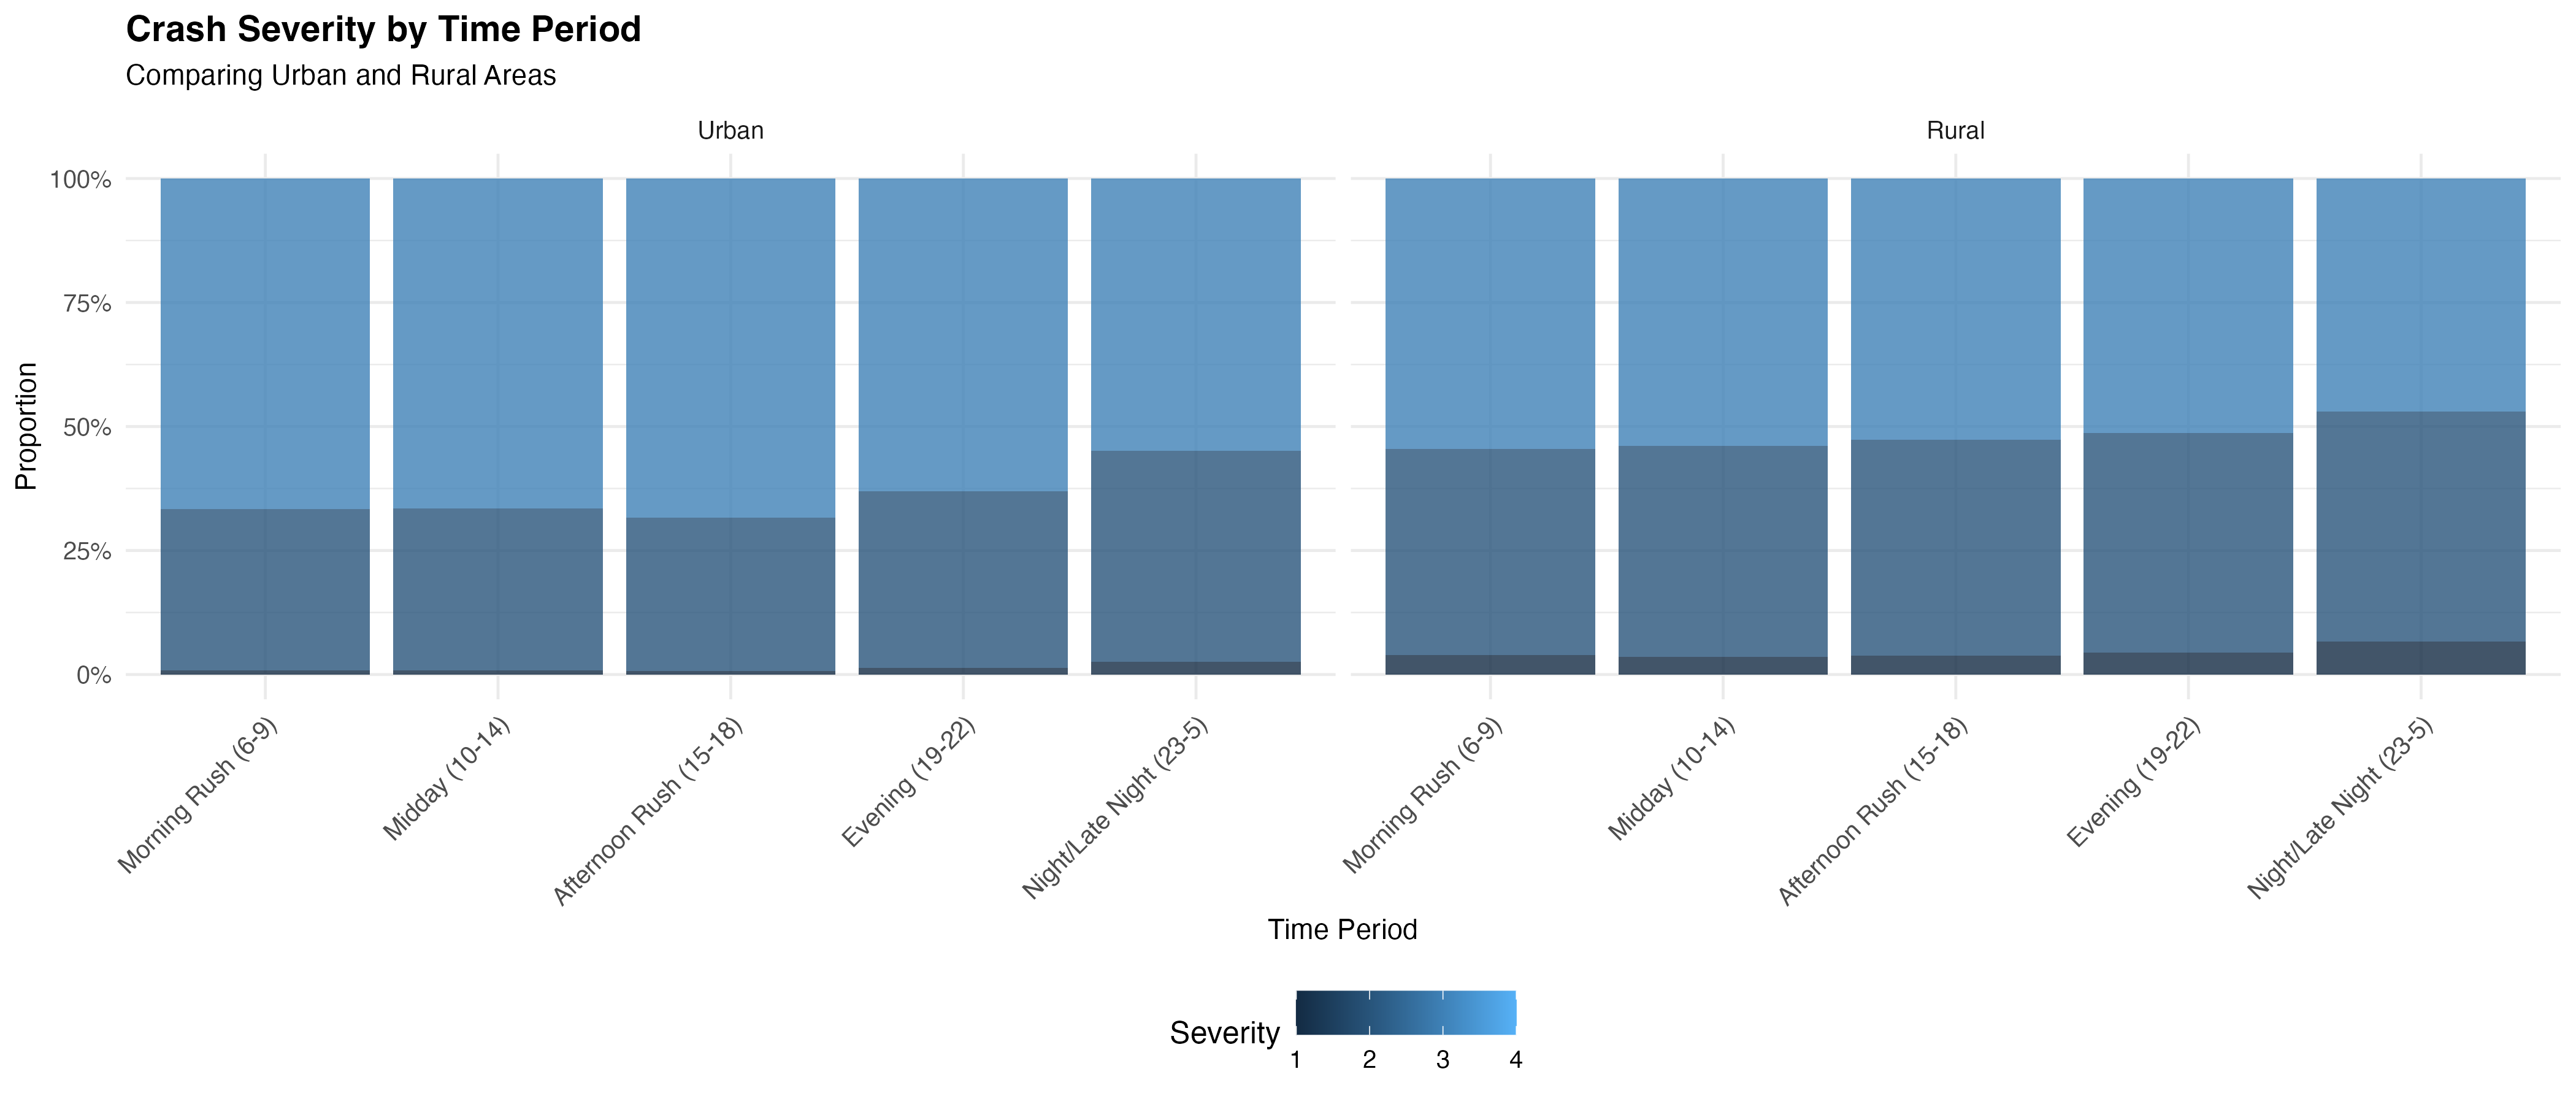
\includegraphics[width=0.7\textwidth]{02_severity_by_time_group_urban_rural.png}
%     \caption{Severity distribution by time period}
%     \label{fig:severity_time}
% \end{figure}

Day of week severity patterns suggest that weekend days show different severity distributions compared to weekdays, with rural areas consistently showing higher severity proportions. % Figure \ref{fig:severity_day} commented for faster compilation

% \begin{figure}[htbp]
%     \centering
%     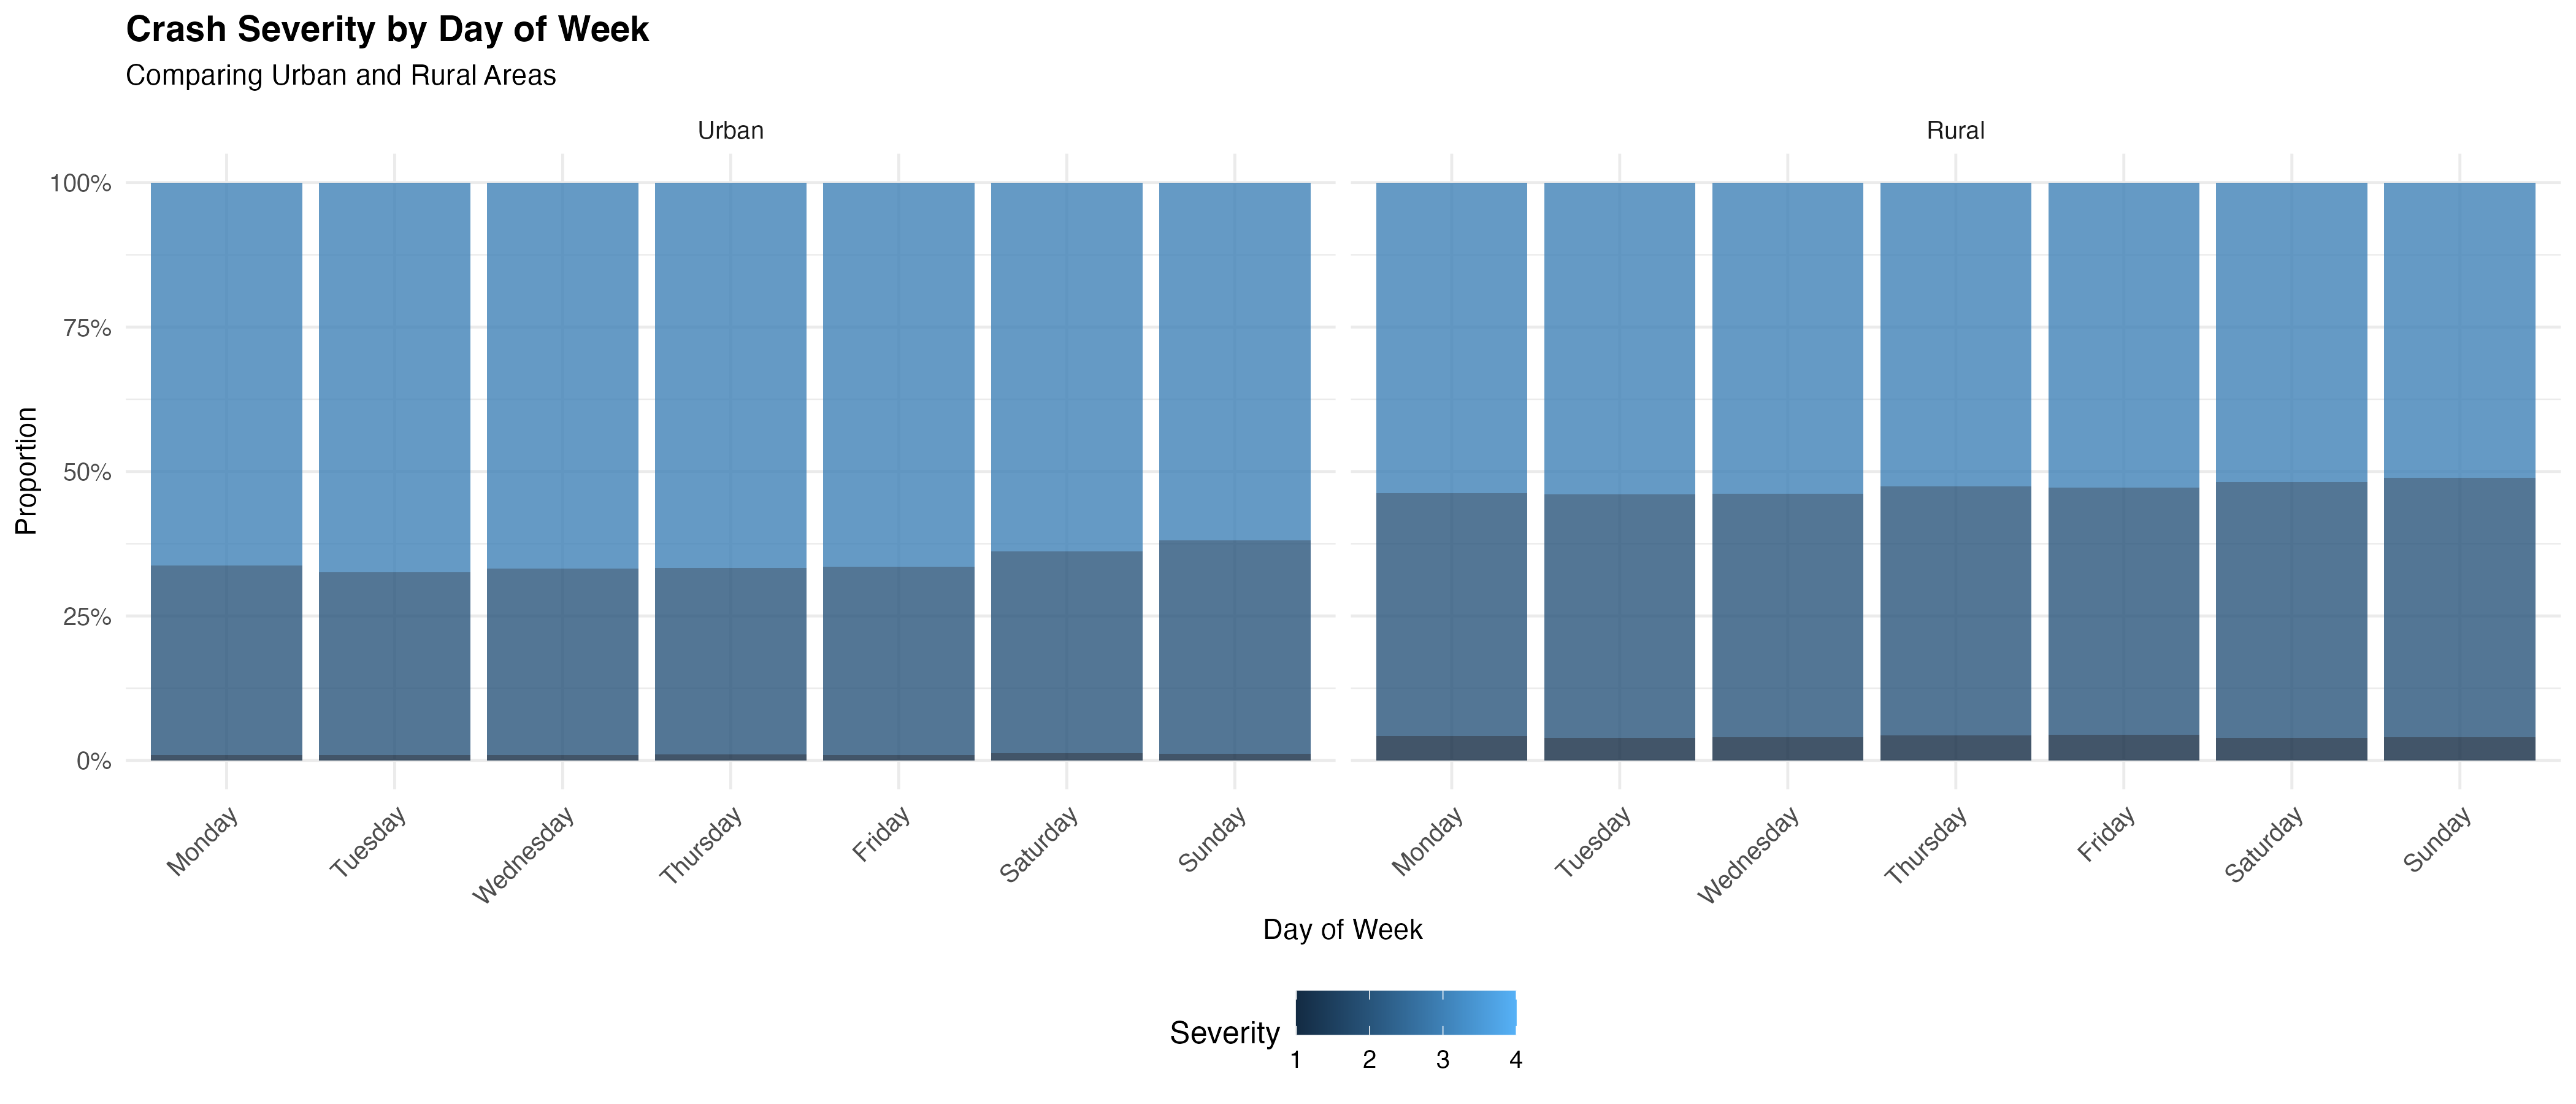
\includegraphics[width=0.7\textwidth]{02_severity_by_day_week_urban_rural.png}
%     \caption{Severity distribution by day of week}
%     \label{fig:severity_day}
% \end{figure}

Seasonal severity variations reveal that winter and spring seasons may have slightly different severity patterns, though these differences are more pronounced in rural areas. % Figure \ref{fig:severity_season} commented for faster compilation

% \begin{figure}[htbp]
%     \centering
%     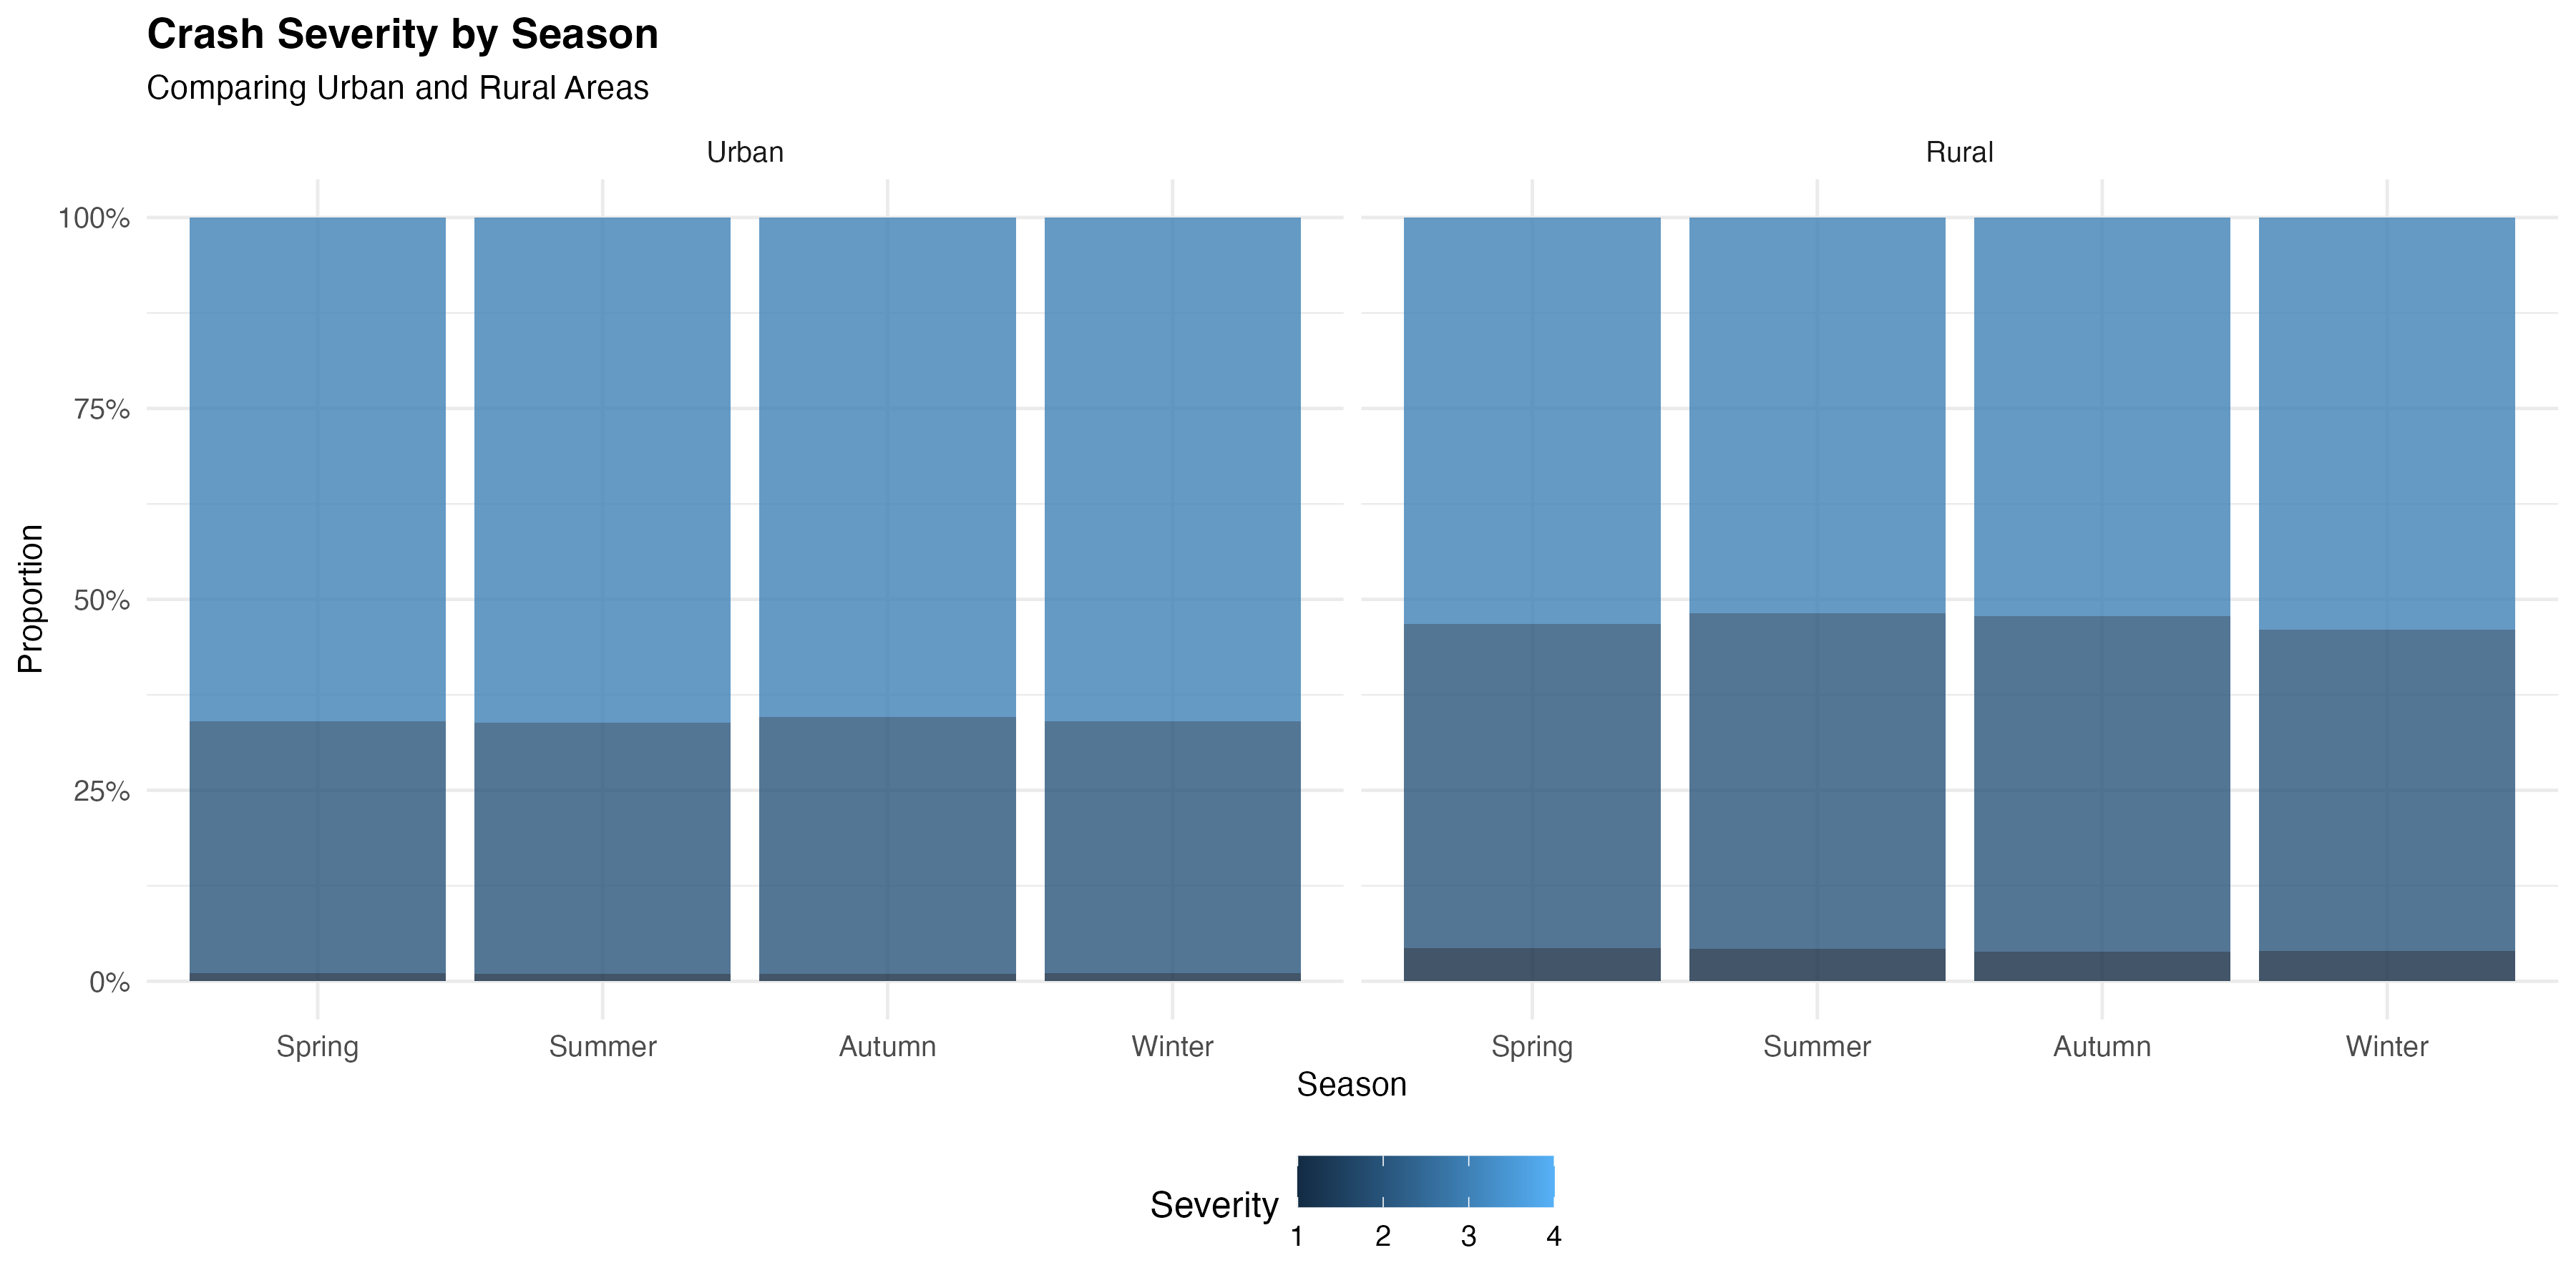
\includegraphics[width=0.7\textwidth]{02_severity_by_season_urban_rural.png}
%     \caption{Severity distribution by season}
%     \label{fig:severity_season}
% \end{figure}

\subsection{Crash Type Analysis}

Crash type distributions show that vehicle-to-vehicle collisions dominate in urban areas, while rural areas exhibit more diverse crash type patterns. % Figure \ref{fig:crash_type} commented for faster compilation

% \begin{figure}[htbp]
%     \centering
%     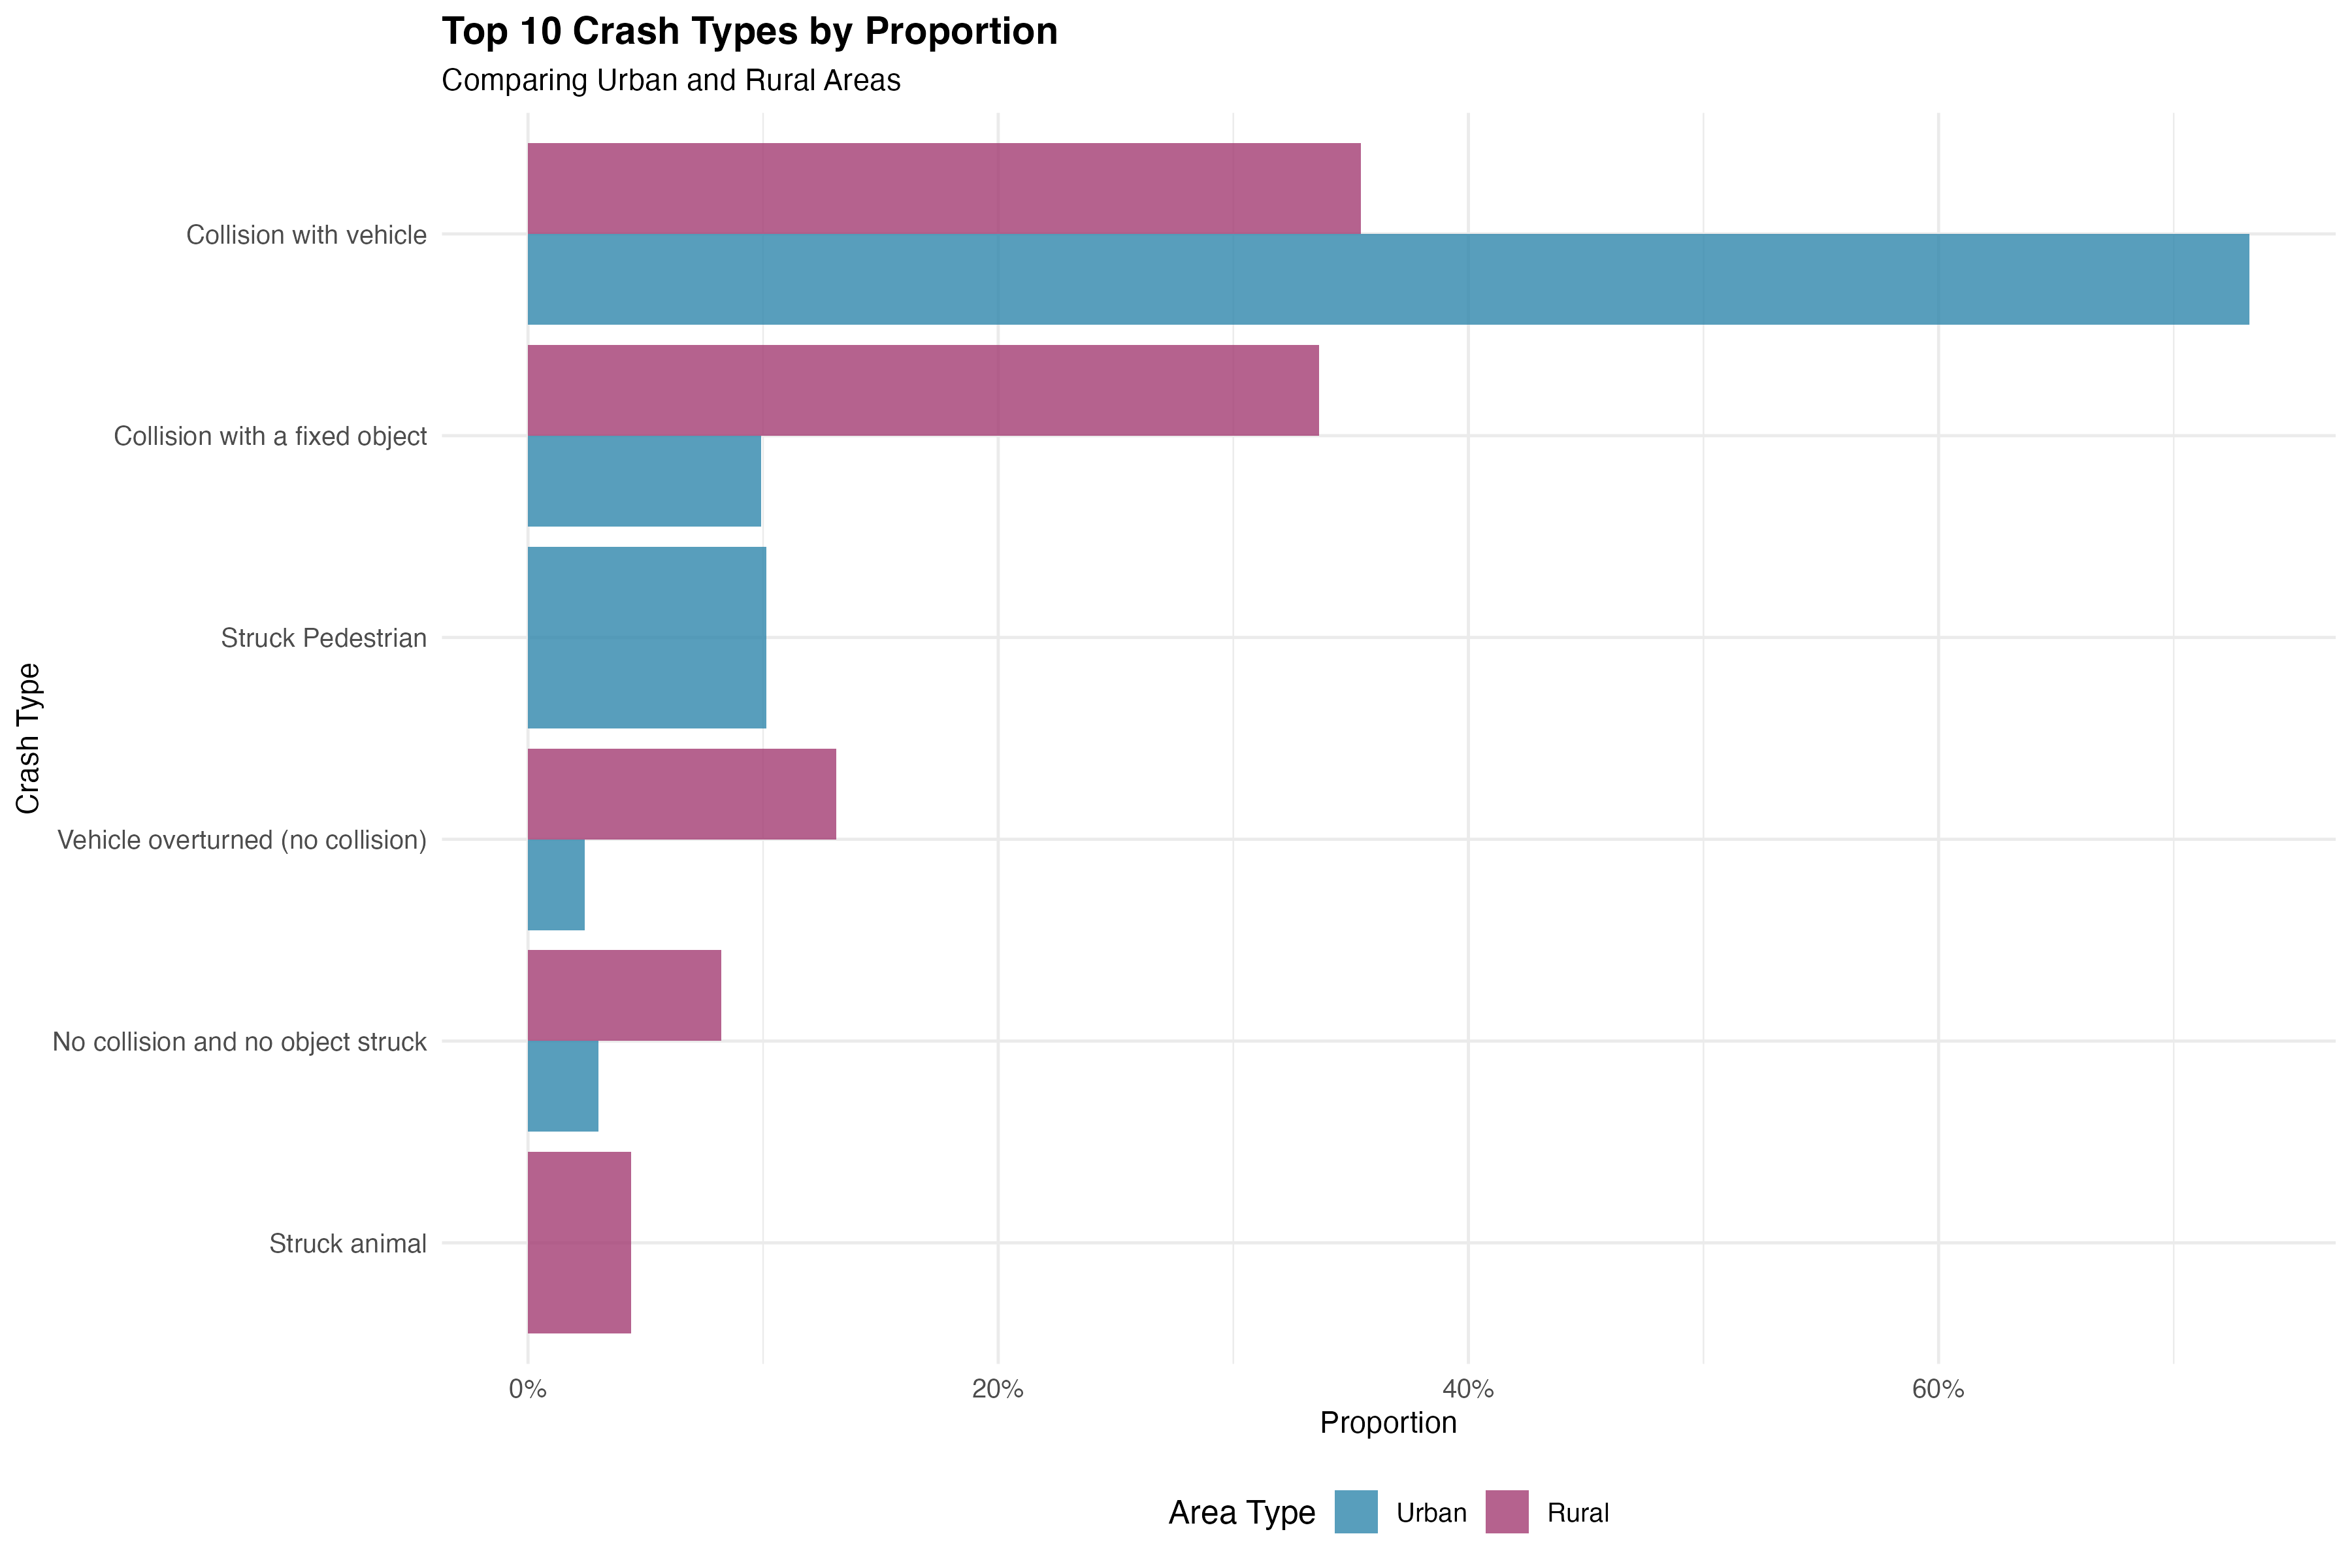
\includegraphics[width=0.7\textwidth]{03_crash_type_distribution_urban_rural.png}
%     \caption{Top crash types comparing urban and rural areas}
%     \label{fig:crash_type}
% \end{figure}

The distribution of crash types by time period reveals that certain crash types are more prevalent during specific time periods, with notable differences between urban and rural contexts. % Figure commented for faster compilation: \ref{fig:crash_type_time}

% \begin{figure}[htbp]
%     \centering
%     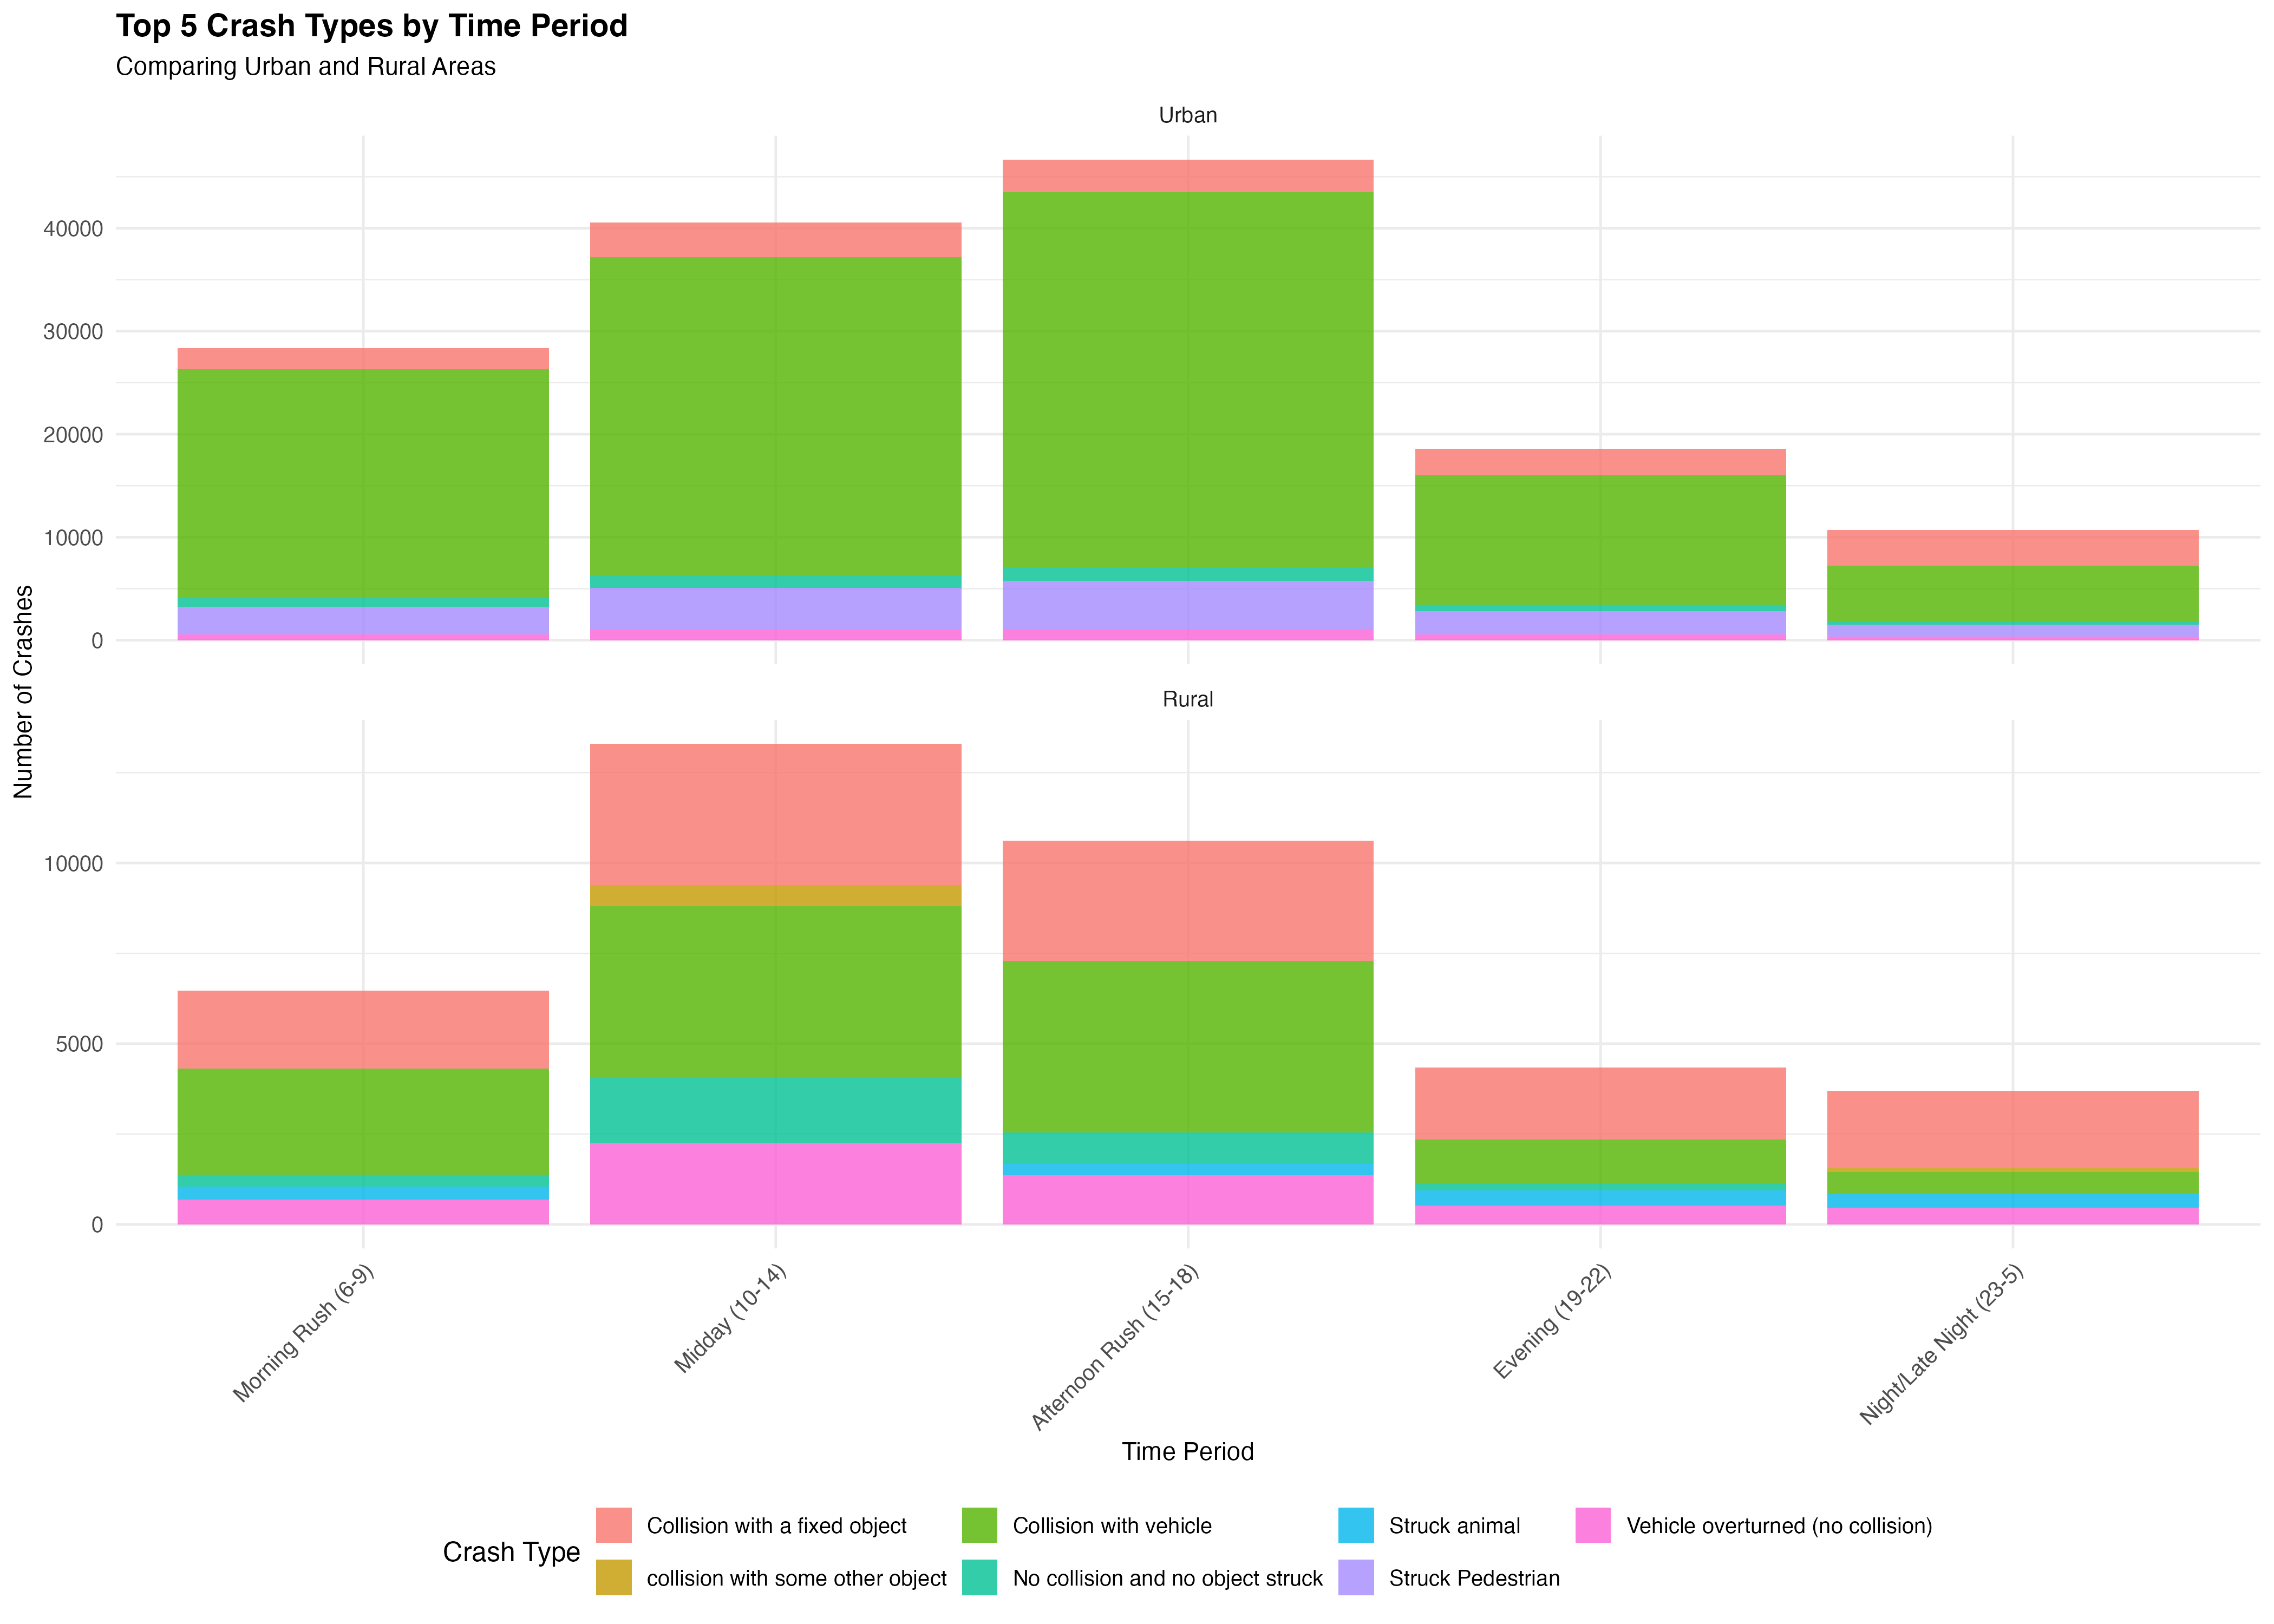
\includegraphics[width=0.7\textwidth]{03_crash_type_by_time_urban_rural.png}
%     \caption{Crash types by time period}
%     \label{fig:crash_type_time}
% \end{figure}

\subsection{Environmental Factors}

Atmospheric conditions show that clear weather dominates crash occurrences, but adverse weather conditions may have different impacts in urban versus rural settings. % Figure \ref{fig:atmospheric} commented for faster compilation

% \begin{figure}[htbp]
%     \centering
%     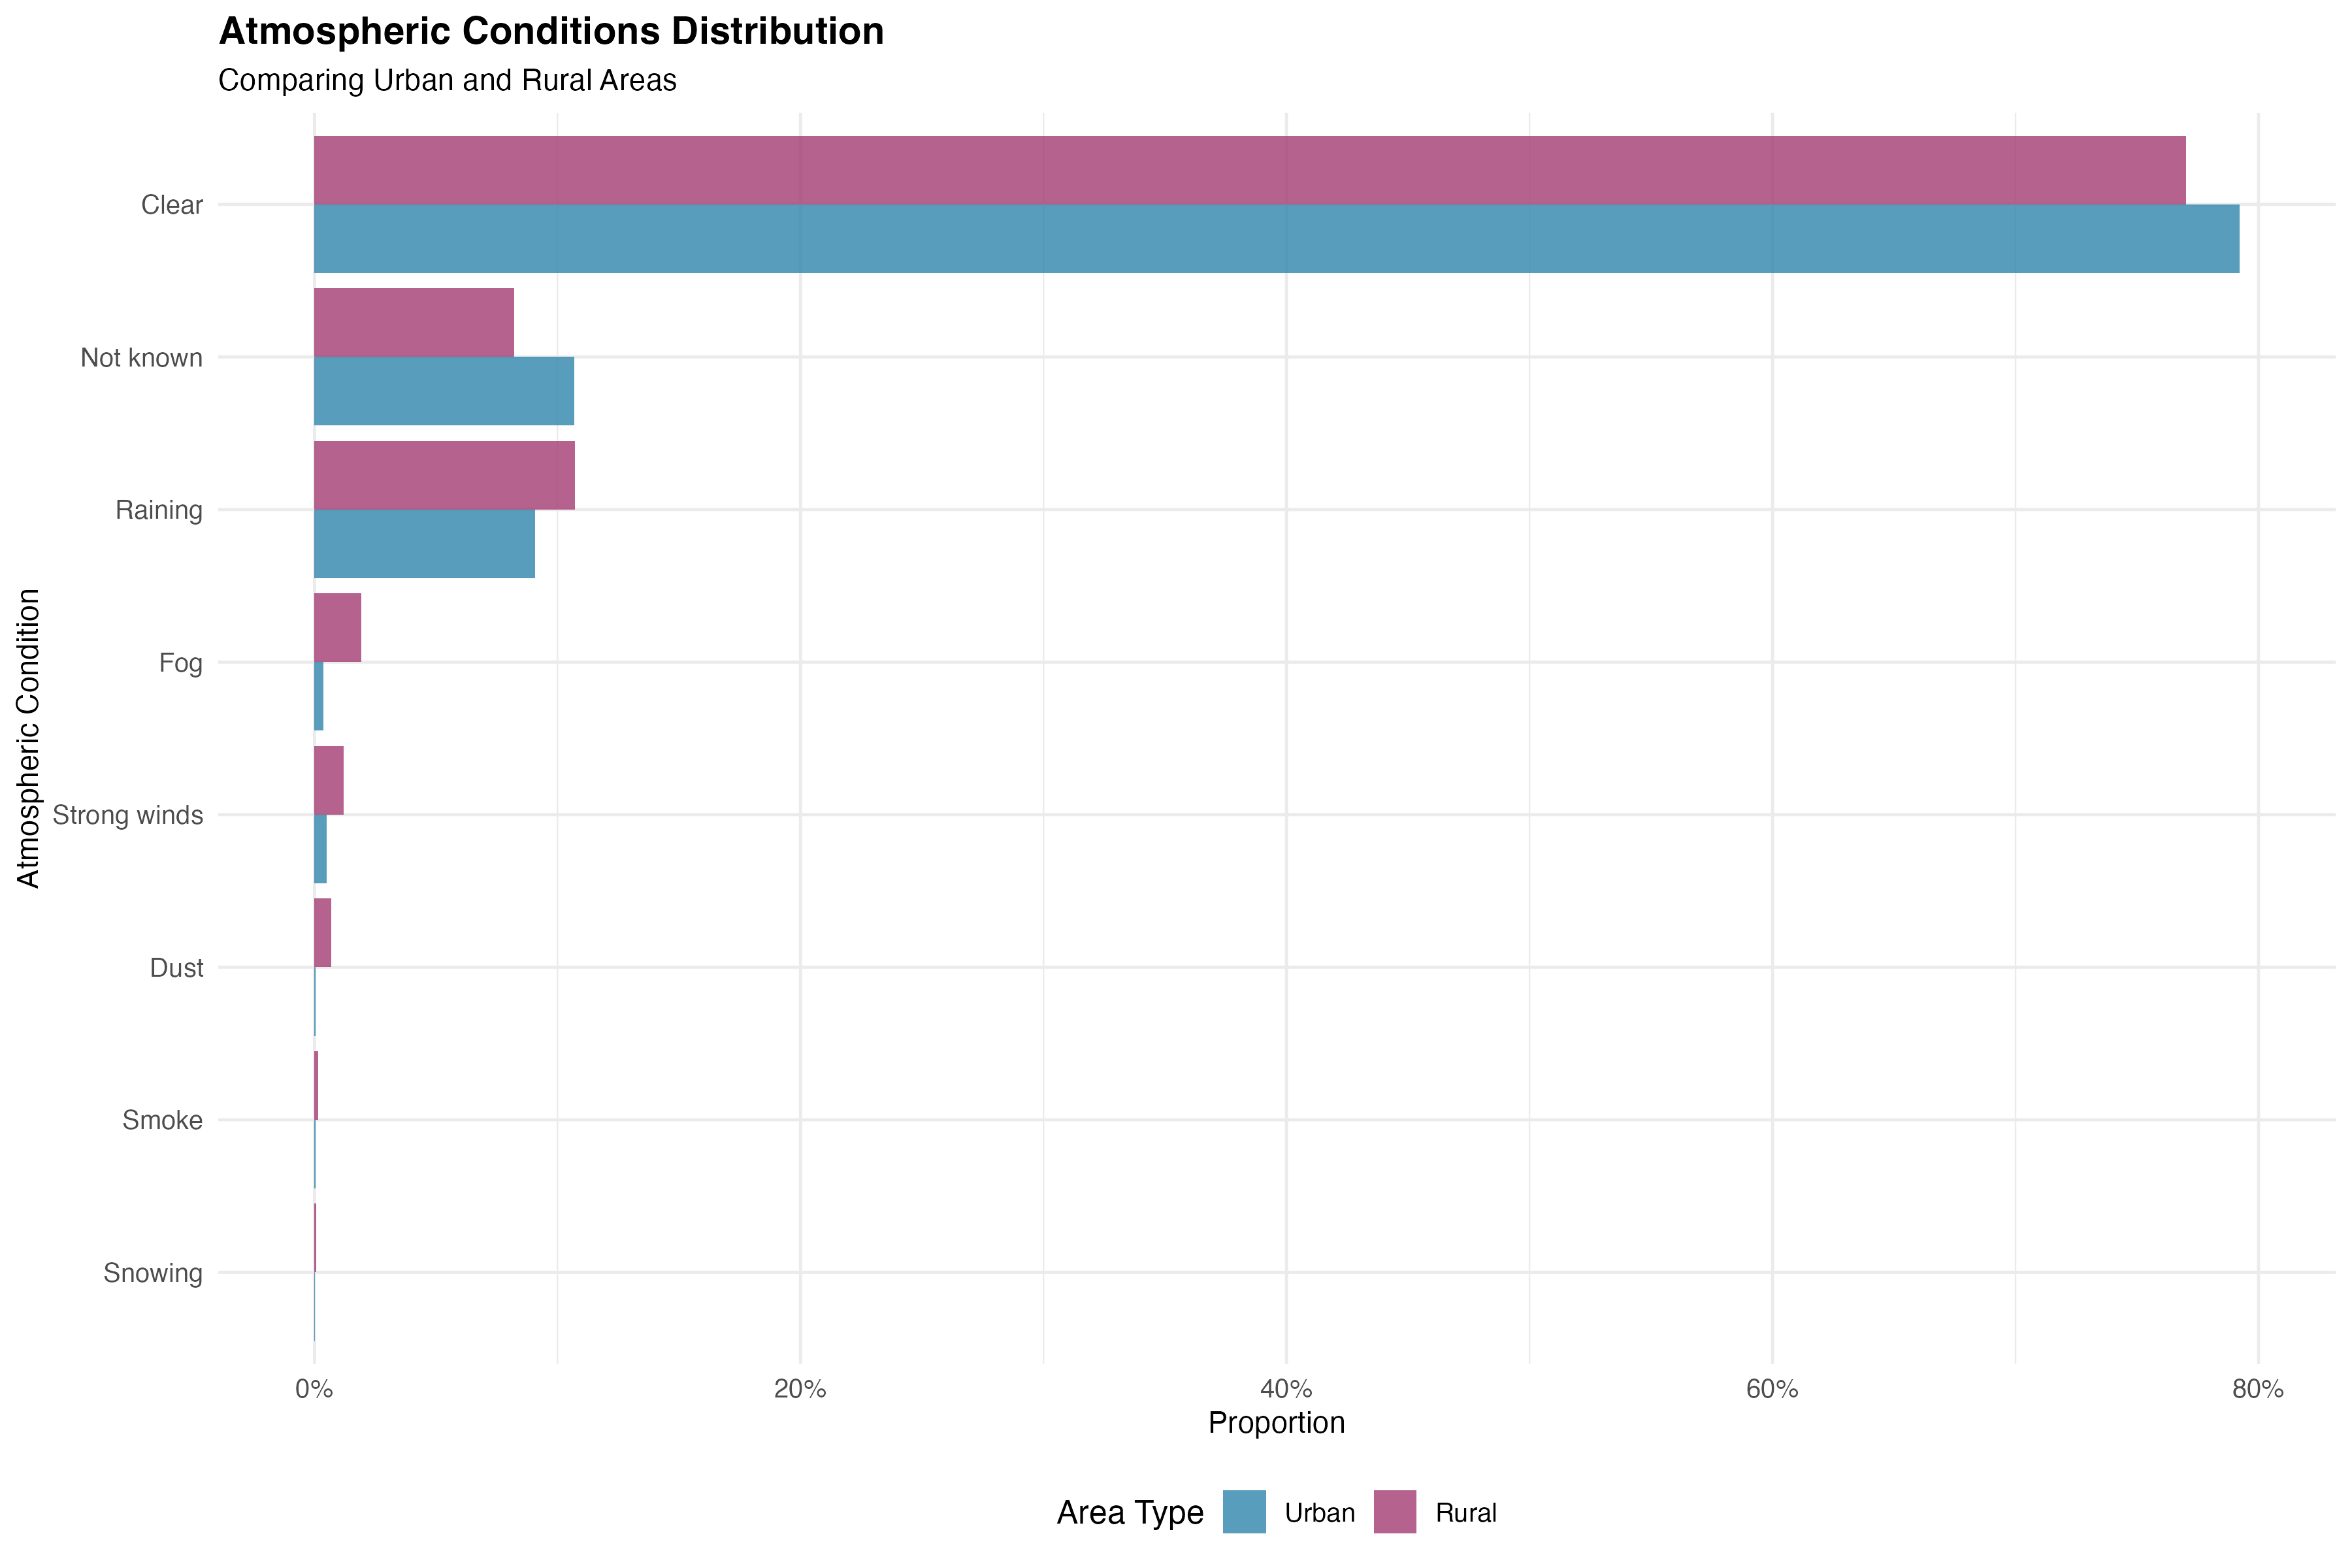
\includegraphics[width=0.7\textwidth]{04_atmospheric_conditions_urban_rural.png}
%     \caption{Atmospheric conditions distribution}
%     \label{fig:atmospheric}
% \end{figure}

Road surface conditions reveal that dry surfaces are most common, but wet and other adverse conditions may contribute differently to crash severity in different area types. % Figure commented for faster compilation: \ref{fig:surface}

% \begin{figure}[htbp]
%     \centering
%     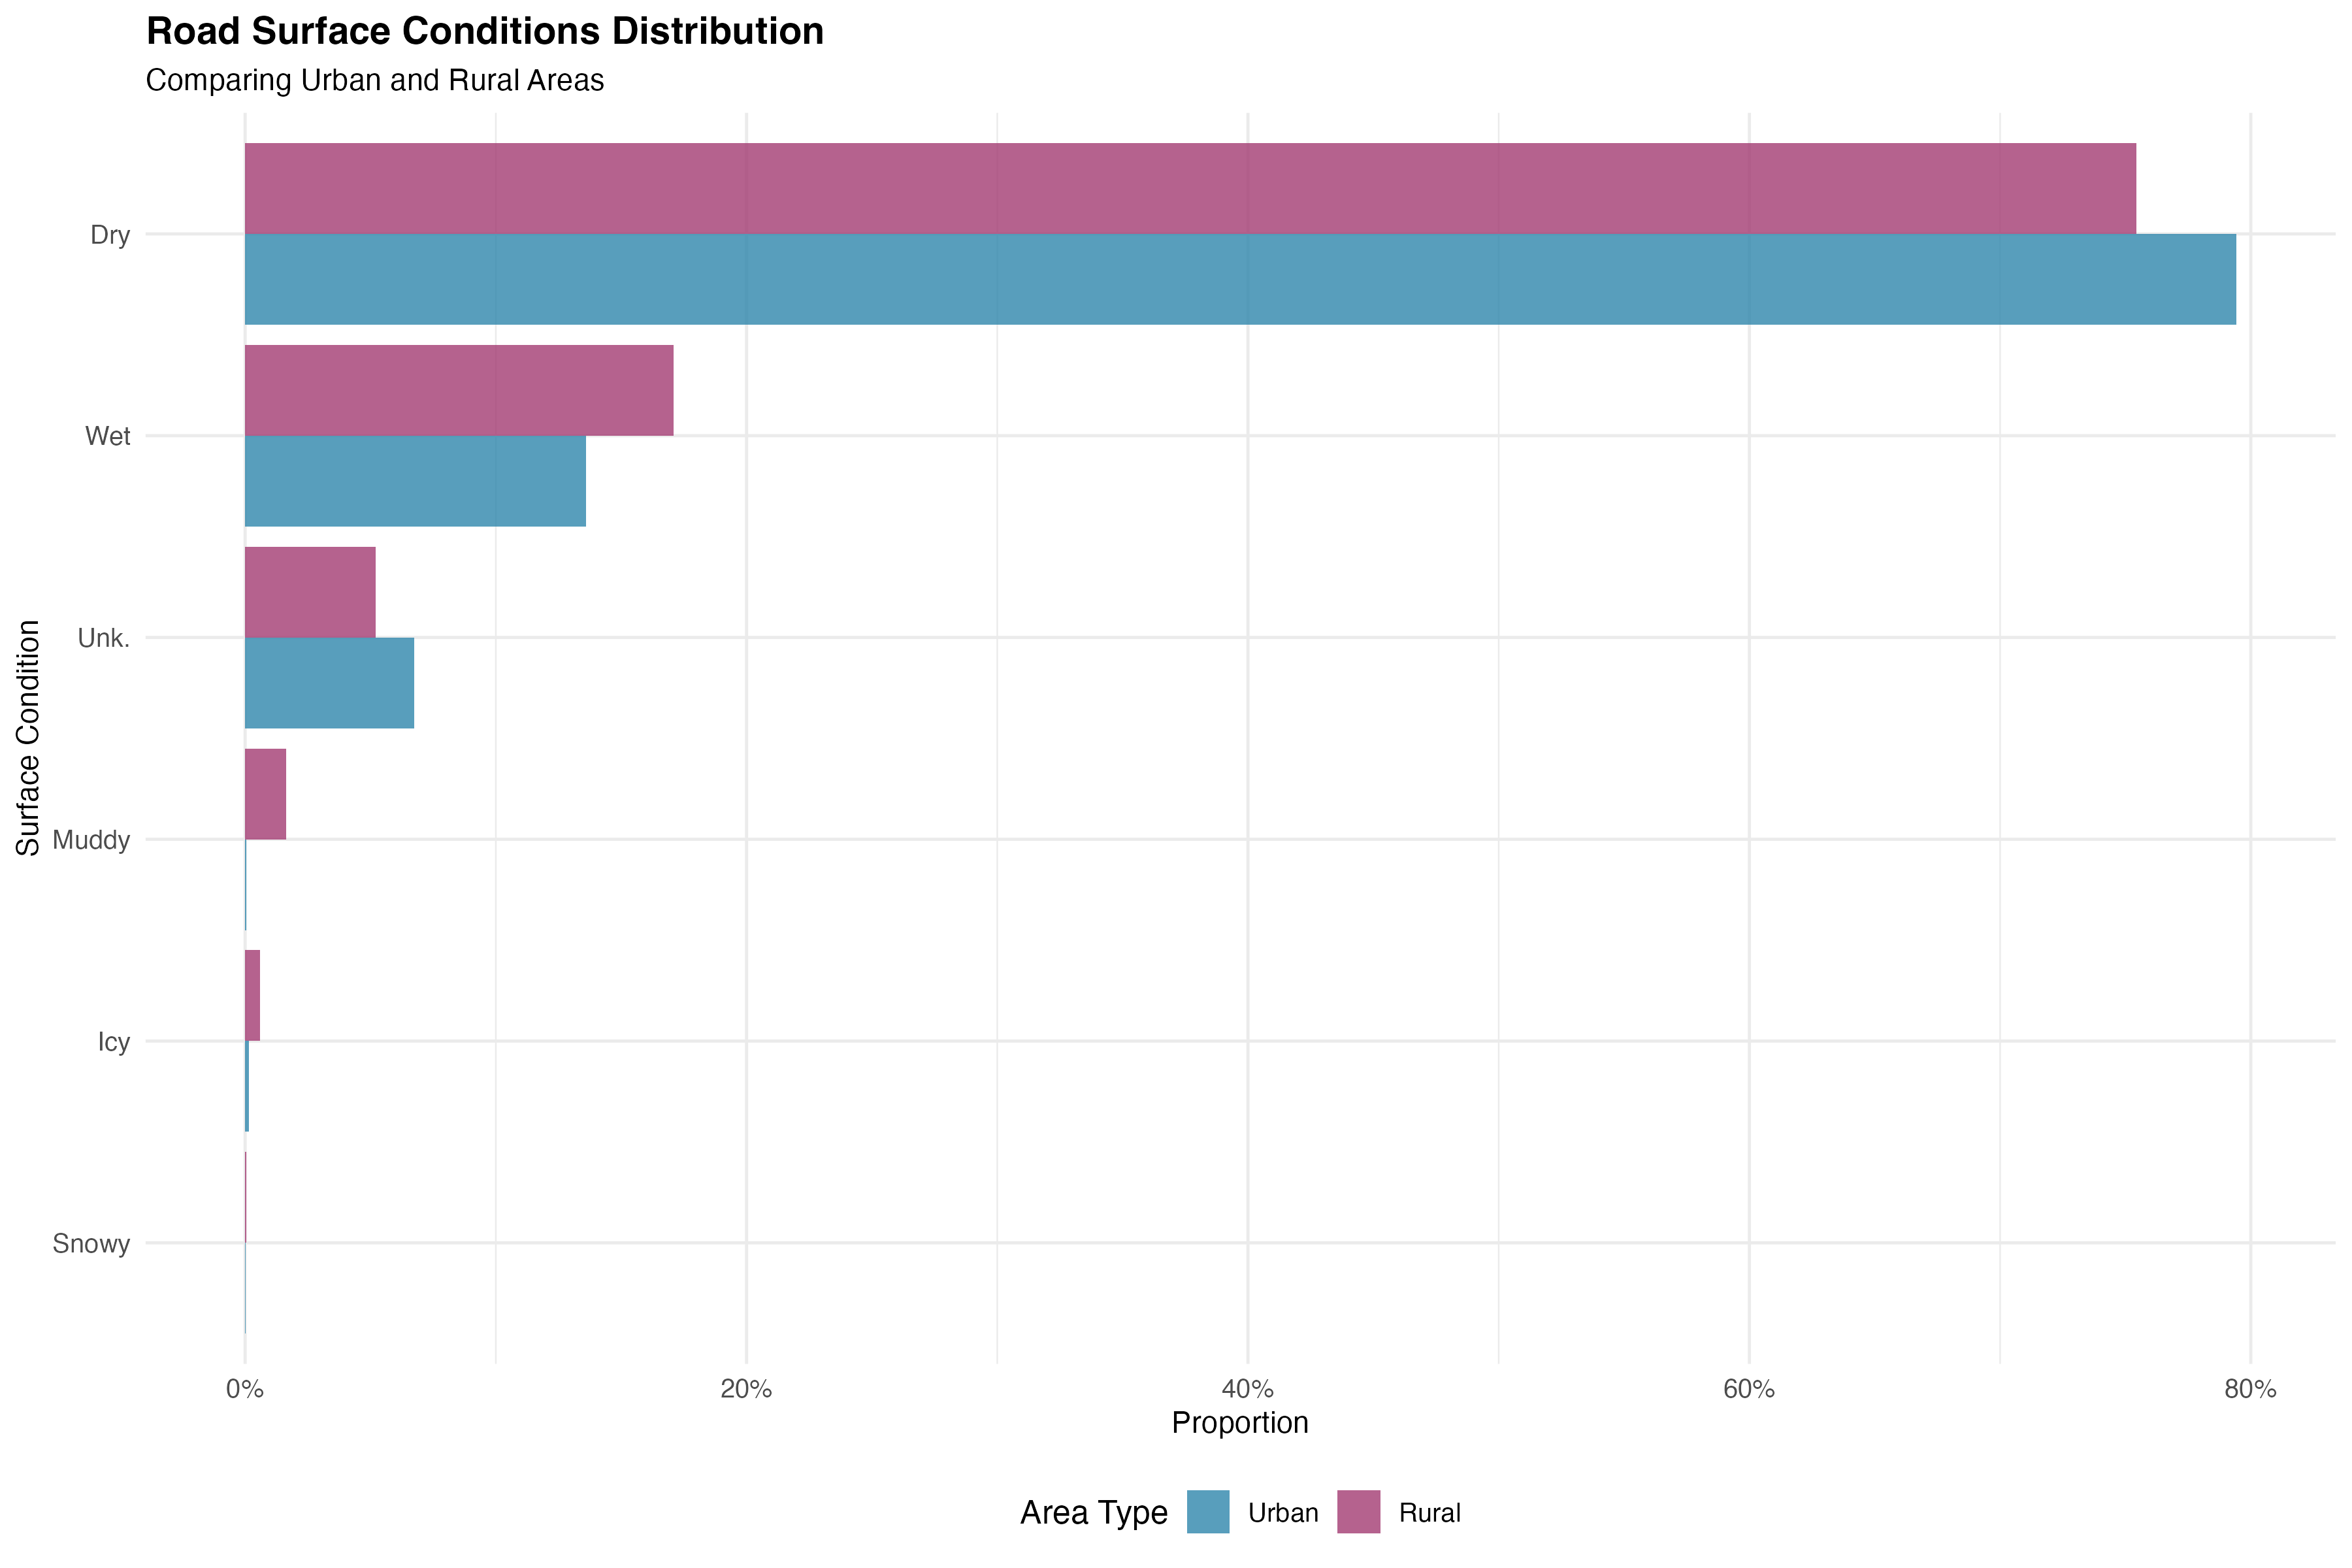
\includegraphics[width=0.7\textwidth]{04_road_surface_conditions_urban_rural.png}
%     \caption{Road surface conditions distribution}
%     \label{fig:surface}
% \end{figure}

The relationship between atmospheric conditions and severity demonstrates how environmental factors influence crash outcomes differently in urban and rural contexts. % Figure commented for faster compilation: \ref{fig:severity_atmos}

% \begin{figure}[htbp]
%     \centering
%     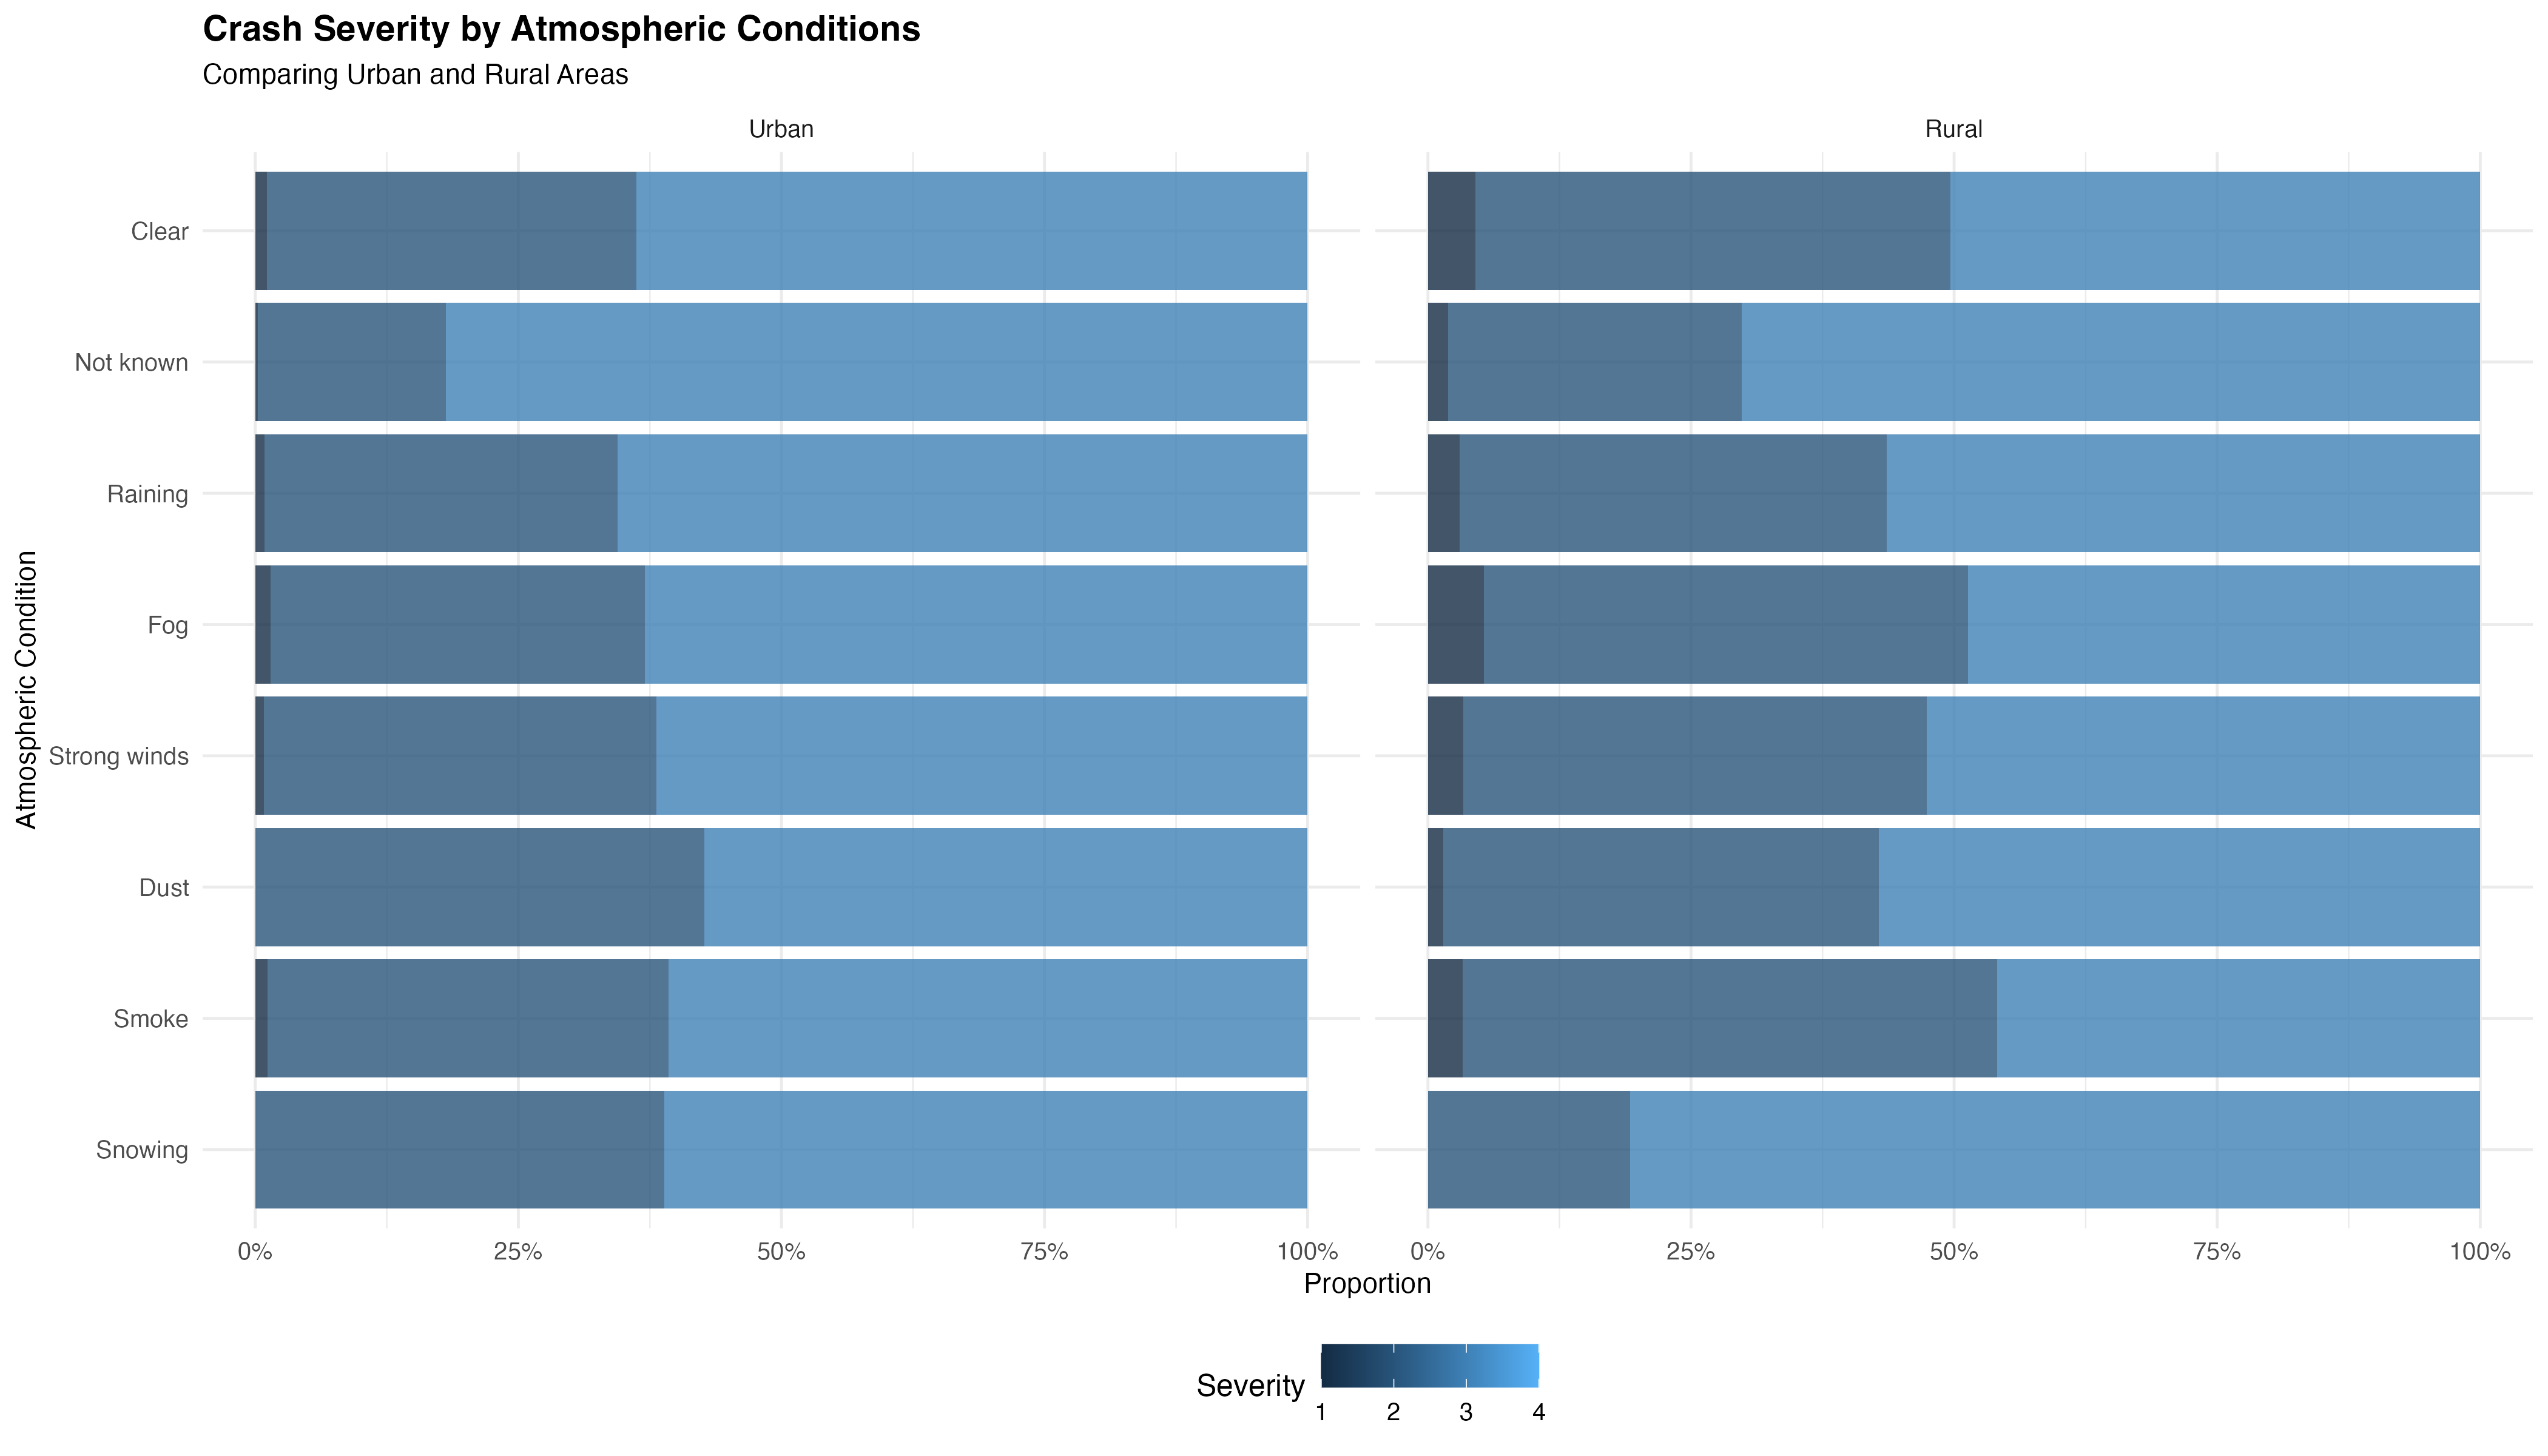
\includegraphics[width=0.7\textwidth]{04_severity_by_atmospheric_urban_rural.png}
%     \caption{Severity by atmospheric conditions}
%     \label{fig:severity_atmos}
% \end{figure}

\section{Statistical Analysis}

\subsection{Frequency Pattern Tests}

Chi-square tests revealed highly significant associations for all temporal patterns:

\begin{itemize}
    \item \textbf{Day of Week}: $\chi^2 = 2368.4$, df = 6, $p < 2.2 \times 10^{-16}$, Cramér's V = 0.113
    \item \textbf{Time Period}: $\chi^2 = 1014.8$, df = 4, $p < 2.2 \times 10^{-16}$, Cramér's V = 0.074
    \item \textbf{Season}: $\chi^2 = 194.82$, df = 3, $p < 2.2 \times 10^{-16}$, Cramér's V = 0.032
\end{itemize}

All tests indicate strong evidence that crash frequency distributions differ significantly between urban and rural areas across temporal dimensions.

\subsection{Severity Analysis Tests}

The severity distribution test showed highly significant differences:
\begin{itemize}
    \item \textbf{Severity Distribution}: $\chi^2 = 3568.5$, df = 3, $p < 2.2 \times 10^{-16}$, Cramér's V = 0.138
\end{itemize}

Fisher's exact test for fatal crash rates revealed:
\begin{itemize}
    \item \textbf{Fatal Crash Rates}: $p < 2.2 \times 10^{-16}$
    \item \textbf{Odds Ratio}: 4.188 (95\% CI: 3.899, 4.500)
    \item Urban fatal rate: 1.01\%
    \item Rural fatal rate: 4.10\%
\end{itemize}

The odds ratio of 4.188 indicates that rural crashes have approximately 4.19 times the odds of being fatal compared to urban crashes, representing a substantial and statistically significant difference.

\subsection{Crash Type Tests}

Chi-square test for crash type distribution:
\begin{itemize}
    \item $\chi^2 = 39,102$, df = 8, $p < 2.2 \times 10^{-16}$, Cramér's V = 0.457
\end{itemize}

The Cramér's V of 0.457 represents a strong association, indicating substantial differences in crash type patterns between urban and rural areas.

\subsection{Environmental Factor Tests}

Both environmental factors showed significant associations:
\begin{itemize}
    \item \textbf{Atmospheric Conditions}: $\chi^2 = 2379.2$, df = 7, $p < 2.2 \times 10^{-16}$, Cramér's V = 0.113
    \item \textbf{Road Surface Conditions}: $\chi^2 = 2750.5$, df = 5, $p < 2.2 \times 10^{-16}$, Cramér's V = 0.121
\end{itemize}

\section{Machine Learning Analysis}

\subsection{Fatal Crash Prediction}

\subsubsection{Logistic Regression Model}
The logistic regression model achieved 98.29\% accuracy in predicting fatal crashes. Key findings from coefficient analysis:
\begin{itemize}
    \item \textbf{Area Type}: Urban area type coefficient = -1.069 ($p < 2 \times 10^{-16}$), indicating significantly lower odds of fatal crashes in urban areas
    \item \textbf{Time Period}: Night/Late Night period showed coefficient = 0.835 ($p < 2 \times 10^{-16}$), indicating higher risk
    \item \textbf{Accident Type}: "Struck Pedestrian" showed the highest positive coefficient (1.161, $p < 2 \times 10^{-16}$), while "Struck Animal" showed strong negative association (-2.852, $p < 4.24 \times 10^{-12}$)
    \item \textbf{Speed Zone}: Higher speed zones (75, 90, 100, 110 km/h) showed positive associations with fatal outcomes
\end{itemize}

\subsubsection{Random Forest Model}
The random forest model achieved identical 98.29\% accuracy, with out-of-bag error estimate of 1.67\%. Feature importance analysis (Figure \ref{fig:rf_importance}) revealed:

% Figure commented for faster compilation - uncomment after successful compile
% \begin{figure}[htbp]
%     \centering
%     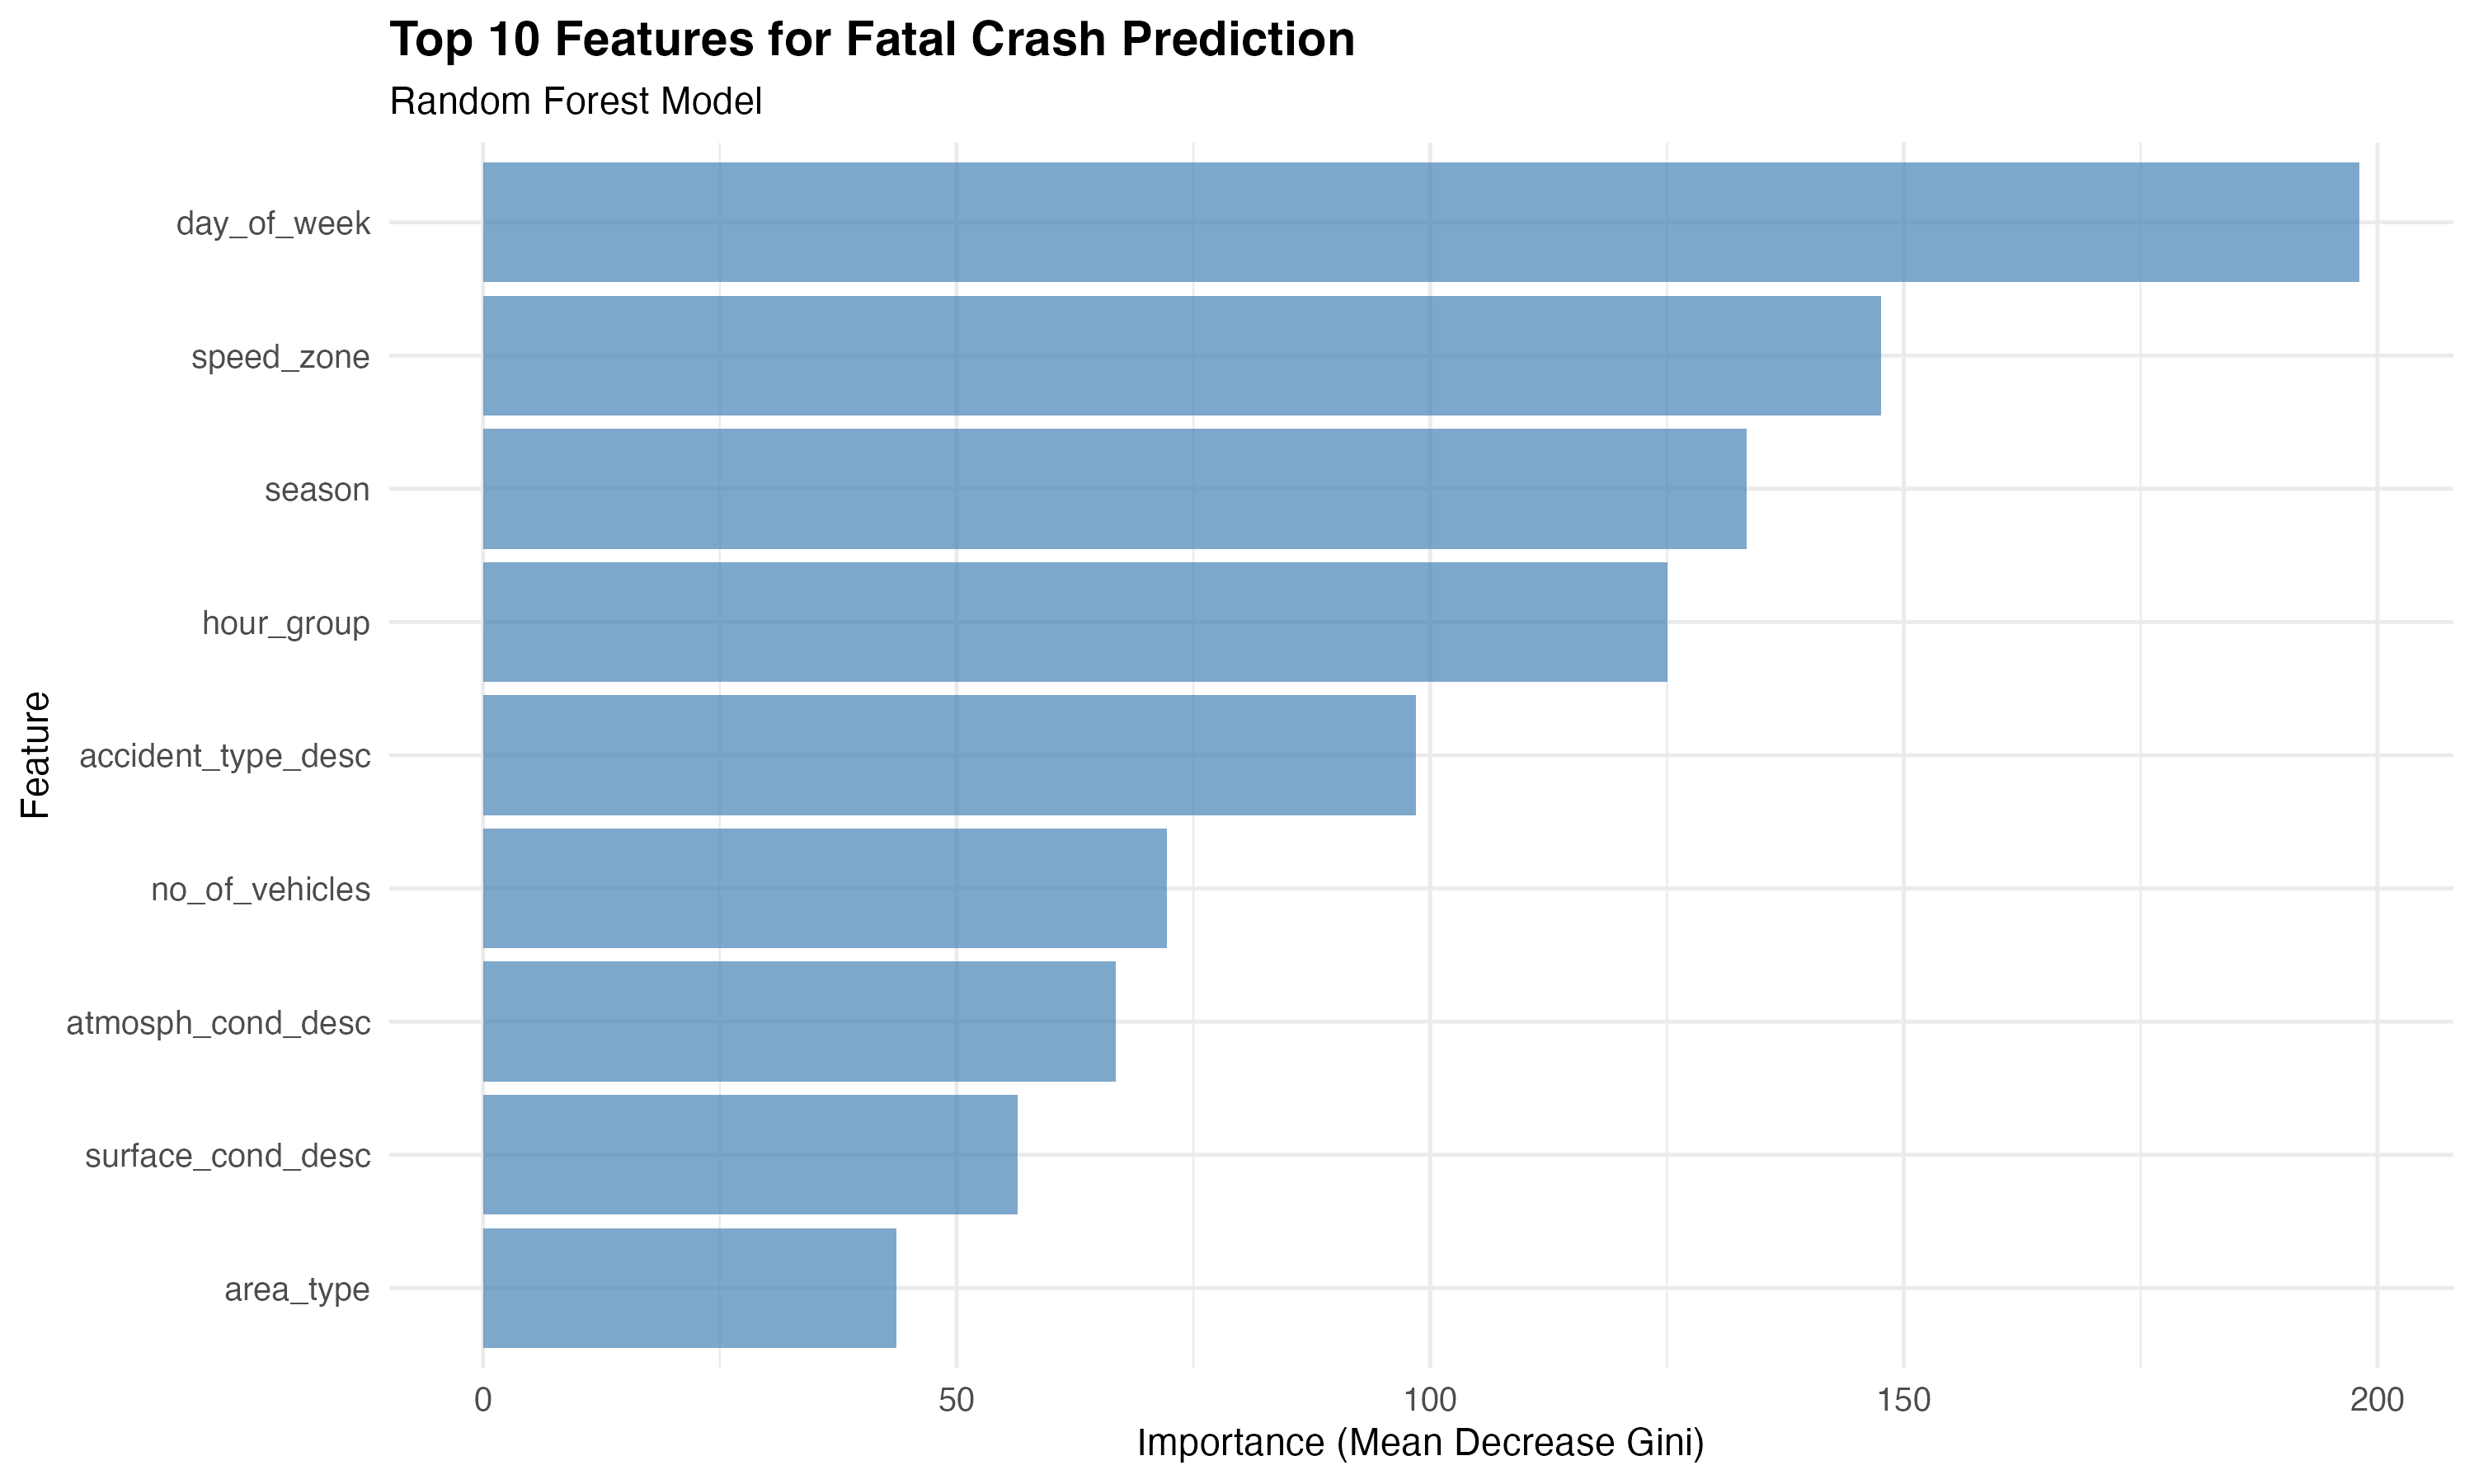
\includegraphics[width=0.7\textwidth]{01_rf_feature_importance.png}
%     \caption{Top 10 features for fatal crash prediction (Random Forest)}
%     \label{fig:rf_importance}
% \end{figure}

The most important features ranked by Mean Decrease Gini:
\begin{enumerate}
    \item Accident type description (98.49)
    \item Day of week (198.12)
    \item Speed zone (147.62)
    \item Season (133.38)
    \item Hour group (125.02)
    \item Number of vehicles (72.18)
    \item Atmospheric conditions (66.77)
    \item Surface conditions (56.45)
    \item Area type (43.64)
\end{enumerate}

\subsection{Severity Category Prediction}

The multi-class random forest model for severity prediction achieved 63.14\% accuracy, with out-of-bag error of 36.74\%. The model demonstrated better performance for minor and serious categories compared to fatal and property damage categories, likely due to class imbalance.

\subsection{Urban vs Rural Separate Models}

Separate models were trained for urban and rural crashes:

\begin{itemize}
    \item \textbf{Urban Model}: 98.94\% accuracy, OOB error = 0.99\%
    \item \textbf{Rural Model}: 95.93\% accuracy, OOB error = 4.13\%
\end{itemize}

Feature importance comparisons revealed:
\begin{itemize}
    \item \textbf{Urban}: Top features were day of week, speed zone, accident type, season, and hour group
    \item \textbf{Rural}: Top features were day of week, speed zone, accident type, hour group, and season
\end{itemize}

While the ordering is similar, the magnitude of importance differs, suggesting different risk factor priorities in urban versus rural contexts.

\subsection{High-Risk Period Identification}

Analysis of fatal crash rates by temporal factors identified:

\textbf{By Time Period (Rural):}
\begin{itemize}
    \item Night/Late Night: 6.59\% fatal rate
    \item Evening: 4.42\% fatal rate
    \item Morning Rush: 3.91\% fatal rate
    \item Afternoon Rush: 3.83\% fatal rate
    \item Midday: 3.61\% fatal rate
\end{itemize}

\textbf{By Day of Week (Rural):}
\begin{itemize}
    \item Friday: 4.44\% fatal rate
    \item Thursday: 4.30\% fatal rate
    \item Monday: 4.23\% fatal rate
    \item Wednesday: 4.00\% fatal rate
    \item Sunday: 3.99\% fatal rate
\end{itemize}

\textbf{By Season (Rural):}
\begin{itemize}
    \item Spring: 4.31\% fatal rate
    \item Summer: 4.24\% fatal rate
    \item Winter: 3.97\% fatal rate
    \item Autumn: 3.86\% fatal rate
\end{itemize}

These findings indicate that rural crashes occurring during night/late night hours on Fridays during spring represent the highest risk combination.

\section{Results and Discussion}

\subsection{Key Findings}

\subsubsection{Urban vs Rural Differences}
The analysis reveals substantial differences between urban and rural crash patterns:
\begin{itemize}
    \item Rural areas experience fatal crash rates approximately 4 times higher than urban areas (4.10\% vs 1.01\%)
    \item Rural areas show higher proportions of serious injuries across all temporal periods
    \item Crash type distributions differ significantly, with rural areas showing more diverse crash scenarios
\end{itemize}

\subsubsection{Temporal Patterns}
Clear temporal patterns emerge:
\begin{itemize}
    \item Afternoon rush hours (15-18) show highest absolute crash frequencies
    \item Night/late night hours show highest fatal crash rates, particularly in rural areas
    \item Friday consistently shows highest crash frequencies and fatal rates
    \item Seasonal variations are present but relatively minor compared to daily and hourly patterns
\end{itemize}

\subsubsection{Risk Factors}
Machine learning analysis identified key risk factors:
\begin{enumerate}
    \item Accident type (especially pedestrian collisions)
    \item Speed zone (higher speeds associated with increased fatal risk)
    \item Area type (rural location is a strong predictor)
    \item Time period (night/late night highest risk)
    \item Number of vehicles involved
\end{enumerate}

\subsection{Model Performance}
The binary classification models for fatal crash prediction demonstrate excellent performance (98.3\% accuracy), though this must be interpreted in context of the severe class imbalance. The models effectively identify key risk factors and can be valuable tools for understanding crash patterns.

The lower accuracy of the multi-class severity prediction model (63.1\%) reflects the complexity of predicting across four severity categories, particularly given the imbalance in class distributions.

\subsection{Limitations}
Several limitations should be acknowledged:
\begin{itemize}
    \item Class imbalance in fatal crashes (1.68\%) may affect model interpretation
    \item Missing data in environmental factors required filtering
    \item Temporal resolution limited by available data granularity
    \item Geographic classification may not capture all urban/rural nuances
    \item Potential confounding factors not captured in the dataset
\end{itemize}

\section{Conclusions}

This comprehensive analysis reveals significant temporal and geographic patterns in crash data from Victoria. Key conclusions include:

\begin{enumerate}
    \item \textbf{Geographic Disparity}: Rural areas face substantially higher fatal crash rates (4x higher odds), indicating a critical need for targeted interventions in rural settings.
    
    \item \textbf{High-Risk Periods}: Night/late night hours, particularly on Fridays during spring, represent the highest risk combinations, especially in rural areas.
    
    \item \textbf{Key Risk Factors}: Accident type (especially pedestrian collisions), speed zone, and area type emerge as the most important predictors of fatal outcomes.
    
    \item \textbf{Model Utility}: Machine learning models achieve high accuracy in fatal crash prediction and provide actionable insights into risk factor prioritization.
    
    \item \textbf{Policy Implications}: Results suggest that interventions should focus on:
    \begin{itemize}
        \item Rural road safety improvements
        \item Night-time driving safety measures
        \item Speed management, particularly in higher speed zones
        \item Pedestrian safety initiatives
    \end{itemize}
\end{enumerate}

\section{Future Work}

Future research directions could include:
\begin{itemize}
    \item Integration of weather data for more comprehensive environmental analysis
    \item Spatial analysis incorporating geographic information system (GIS) data
    \item Longitudinal analysis to examine temporal trends over years
    \item Incorporation of traffic volume data to normalize crash rates
    \item Development of real-time prediction systems for high-risk periods
\end{itemize}

\section{Acknowledgments}

This analysis utilized crash data from Victoria, Australia. All analyses were conducted using R statistical software with appropriate packages for data manipulation, visualization, statistical testing, and machine learning.

\end{document}

